% \section{Background}
\label{sec:vibvoice_background}
This section introduces EarSense, an open-source wearable platform with a sensing setup similar to current commercial HMWs (Section~\ref{sec:vibvoice_EarSense}). It then analyzes bone-conducted vibration and audio signals recorded by EarSense under several settings (Section~\ref{sec:vibvoice_measurement}). Finally, it summarizes the VibVoice design (Section~\ref{sec:vibvoice_overview}) and introduces the Bone Conduction Function and multimodal network (Sections~\ref{sec:vibvoice_bcf} and~\ref{sec:vibvoice_network}).


\subsection{EarSense: An Open Source Data Collection Platform for HMWs}
\label{sec:vibvoice_EarSense}

Most commercial HMWs do not provide APIs to collect raw acceleration data. Apple provides APIs~\citep{CMHeadph3:online} for collecting AirPods motion data at $100\,\text{Hz}$, but this sampling rate is too low for speech-related vibration and does not fully use the commercial IMU.
We therefore develop a sensing platform that can: a) collect acceleration and acoustic data synchronously at a sample rate suitable for speech information; b) maintain contact with the user's head in a manner similar to HMWs; and c) remain compatible with existing commercial devices.
\begin{figure}
  \begin{subfigure}{.64\columnwidth}
    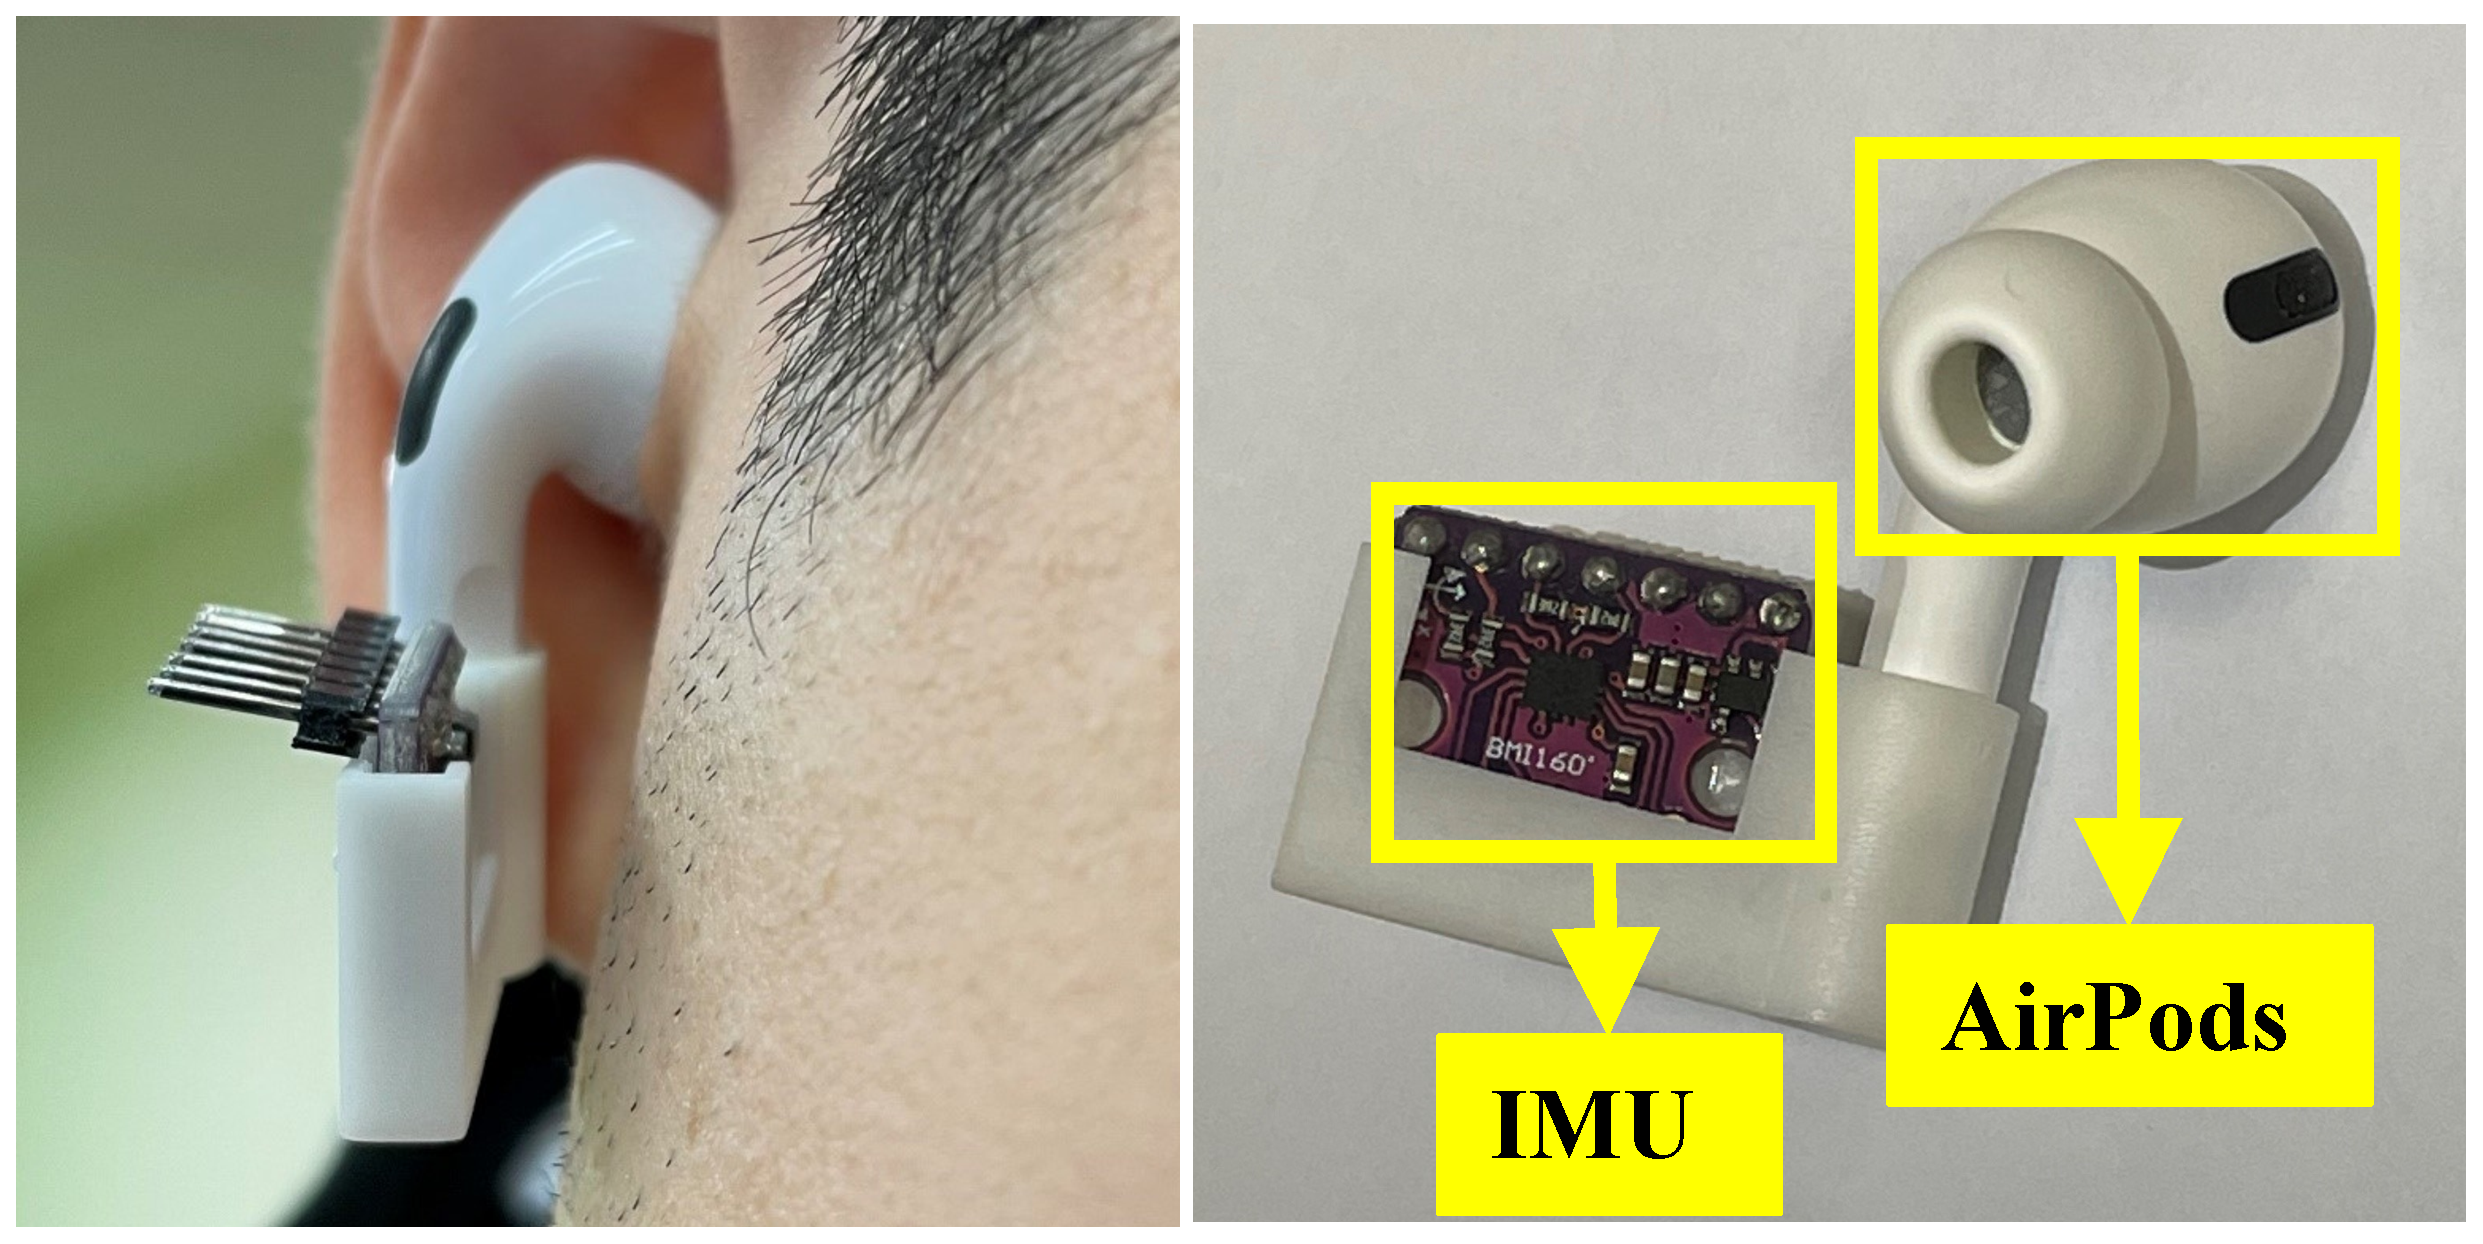
\includegraphics[width=\textwidth]{chapters/vibvoice/figure/earsense.eps}
    \caption{\emph{EarSense} with an Airpods Pro.}
    \label{fig:vibvoice_earsense-head}
  \end{subfigure}
  \begin{subfigure}{0.35\columnwidth}
    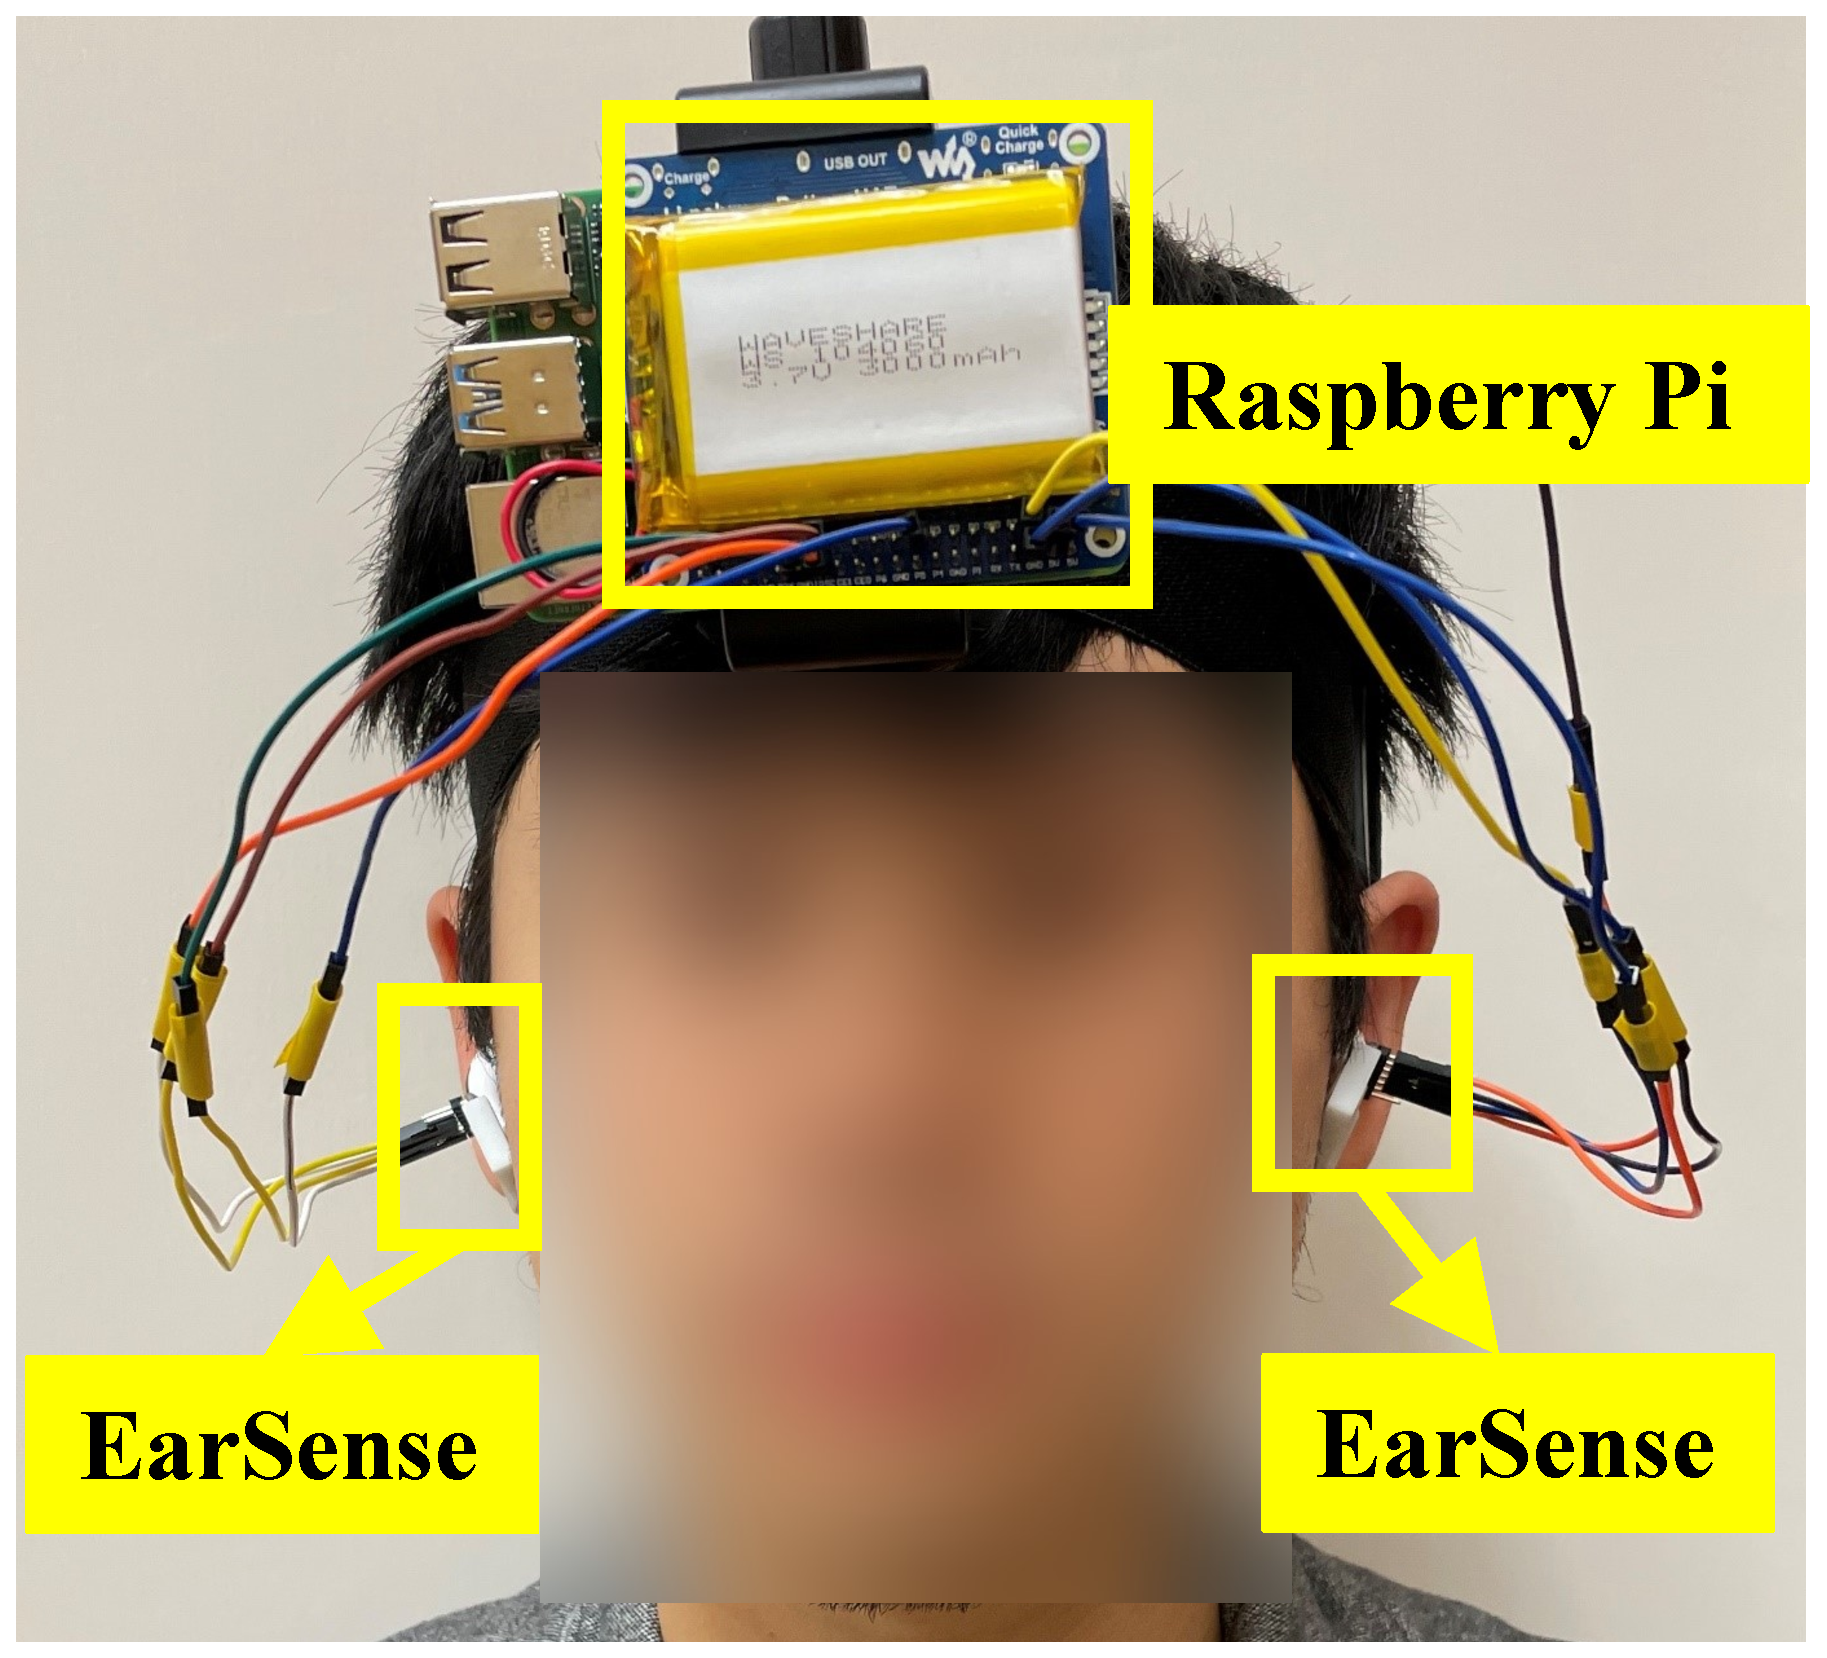
\includegraphics[width=\textwidth]{chapters/vibvoice/figure/people.eps}
    \caption{Test Setup.}
    \label{fig:vibvoice_earsense-people}
  \end{subfigure}
  \caption{\emph{EarSense} is an open-sourced data collector attachable to commercial HMWs for vibration sensing.}
  \label{fig:vibvoice_earsense}
\end{figure}

Fig. \ref{fig:vibvoice_earsense} shows the prototype of \textit{EarSense}  \citep{dataset}, a new open-sourced sensing platform that equips a 3D-printed enclosure with an IMU sensor (i.e., Bosch BMI-160 \citep{Inertial63:online}) inserted. EarSense has a flexible design to make it attachable to any commercial HMW device (e.g., AirPods Pro). EarSense captures the same vibration as the testing HMW and has no direct contact with the user's head (shown in Fig. \ref{fig:vibvoice_earsense-head}).
We connect two EarSenses to a Raspberry Pi (RPi) with a battery for data collection.
Fig. \ref{fig:vibvoice_earsense-people} shows a volunteer wearing the device on the head to avoid excessive vibrations caused by the connecting wires.
A Python script on the RPi controls the EarSense devices through the I2C protocol and stores the data for offline processing.
We only use the three-axis accelerometer provided by the IMU chip because the gyroscope and magnetometer are less related to the vibration.
The default sample rates of the microphone and accelerometer are $16\,\text{kHz}$ and $1.6\,\text{kHz}$, respectively. Since commercial earphones such as AirPods Pro do not support two-channel audio recording through public APIs, EarSense records audio in a mono channel.
We apply L2-Norm to the spectrograms of three-axis acceleration to extract the vibration intensity and avoid the impact of wearing position and user's motion.

\subsection{Measurements of Bone-Conducted Vibrations}
\label{sec:vibvoice_measurement}
We measure the difference between audio and bone-conducted vibrations with EarSense under various settings, i.e., the noises caused by the competing speaker and user motion. In each experiment, we ask a volunteer to wear Apple AirPods Pro with EarSense attached (shown in Fig. \ref{fig:vibvoice_earsense-people}) in a meeting room with the size of $10~\text{m}^2$. 
\begin{figure}
    \begin{subfigure}{0.46\columnwidth}
        \centering
        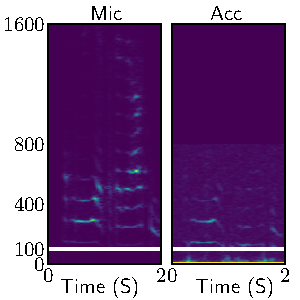
\includegraphics[width=1\textwidth]{chapters/vibvoice/figure/clean.pdf}
        \caption{The user is talking with no noise.}
        \label{fig:vibvoice_nospeaker}
        \end{subfigure}
        \hspace{.5em}
    \begin{subfigure}{0.46\columnwidth}
        \centering
        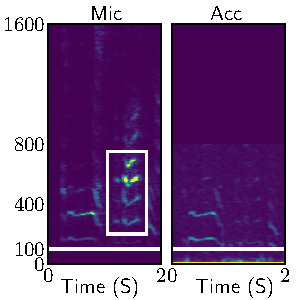
\includegraphics[width=1\textwidth]{chapters/vibvoice/figure/noise.pdf}
        \caption{The user is talking with a competing speaker.}
        \label{fig:vibvoice_speaker}
         \end{subfigure}
    \caption{Impact of the competing speaker.}
    \label{fig:vibvoice_competing-speaker}
\end{figure}

\noindent\textbf{Competing speaker.}
First, we ask the user to sit in the meeting room and speak while a loudspeaker is playing a pre-recording speech one meter from the user as the competing speaker. Note that the competing speaker is one of the most challenging environmental noises for HMWs since its spectrum is similar to the speech's, making it indistinguishable from the noise suppression algorithms. 
We set the volume of the competing speaker to be similar to the user, in which SNR is 3 dB. It is difficult to separate the two sources according to volume since the two speeches are mixed.
Fig. \ref{fig:vibvoice_nospeaker} and Fig. \ref{fig:vibvoice_speaker} show the spectrograms of microphone audio and acceleration when the environment is quiet or contains a competing speaker when the user is talking, respectively.
Note that we only show the spectrogram up to $1.6\,\text{kHz}$ since there is slim energy in the frequency bands higher than $1.6\,\text{kHz}$ of the microphone, and the accelerometer can only sense the signal with a frequency band of $800\,\text{Hz}$.
The spectrograms show that acceleration has lower signal energy than microphone audio since acoustic vibration attenuates during bone conduction, especially for high-frequency vibrations. Compared with the silent environment, the audio spectrogram of microphone audio with a competing speaker shows strong distortions, as highlighted with the white box in Fig. \ref{fig:vibvoice_speaker}. However, the accelerometer spectrograms do not show this phenomenon because the competing speaker cannot produce bone-conducted vibrations.
In summary, the accelerometer receives the user's voice through bone conduction only, excluding environmental sounds over the air, which is ideal for speech enhancement.

\noindent\textbf{User motion.}
We also measure the noises caused by the user's motion. We ask the volunteer to walk while talking. Fig. \ref{fig:vibvoice_walk} shows that walking causes low-frequency noises in the acceleration. The green boxes show the zoom-in result of the signals below $100\,\text{Hz}$. We can observe clear periodic fluctuations in low frequency (i.e., $< 50\,\text{Hz}$), which are caused by the steps of the volunteer.
In summary, the user's motion only affects the acceleration at lower frequencies, which does not affect our speech enhancement.
In addition, we observe slight low-frequency fluctuation in acceleration in Fig. \ref{fig:vibvoice_competing-speaker}, although the volunteer is asked to stand still in this experiment. Since most of the human speech is above $85~\text{Hz}$ \citep{Voicefre75:online}, the removal of audio in low frequency (i.e., the white horizontal lines in Fig. \ref{fig:vibvoice_competing-speaker}) can effectively reduce the interference caused by human motion.

\begin{figure}
\begin{minipage}[t]{0.46\columnwidth}
     \centering
        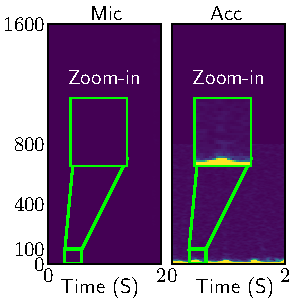
\includegraphics[width=1\textwidth]{chapters/vibvoice/figure/notalk.pdf}
        \caption{Spectrograms of microphone and acceleration when the user is walking.}
        \label{fig:vibvoice_walk}
\end{minipage}
\hfill
   \begin{minipage}[t]{0.48\columnwidth}
     \centering
       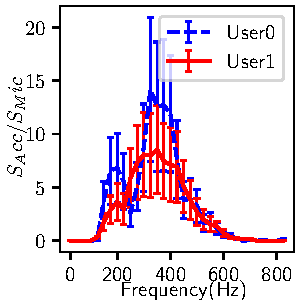
\includegraphics[width=1\textwidth]{chapters/vibvoice/figure/transfer_variance.pdf}
    \caption{Frequency responses of two users' bone-conducted vibrations.}
    %\vspace{-2em}
    \label{fig:vibvoice_bcf}
\end{minipage}
\end{figure}

\noindent\textbf{Frequency Response.}
We further explore the frequency response of bone-conducted vibrations among users. 
Specifically, we measure the frequency response of bone-conducted vibrations as follows: First, we compute the spectrums of audio and vibration data, which is denoted by $S_{Mic}$ and $S_{Acc}$, respectively. Then, we compute the Bone Conduction Function denoted by the frequency response of bone-conducted vibrations by $S_{Acc}/S_{Mic}$ at every frequency band. Fig. \ref{fig:vibvoice_bcf} shows two volunteers' frequency responses, in which the error bars represent the averages and variances.
The acceleration shows higher sensitivity than the microphone within the frequency of $200\text{Hz}\sim500\text{Hz}$, while lower sensitivity at a higher frequency ($>500\text{Hz}$) due to the absorption by the head skull. 
In addition, the frequency response keeps significant similarity among users, indicating the generalization to other users.
Hence, the Bone Conduction Function should consider inter-people diversity and inter-people similarity.

\begin{figure}
\begin{minipage}[t]{0.48\columnwidth}
     \centering
    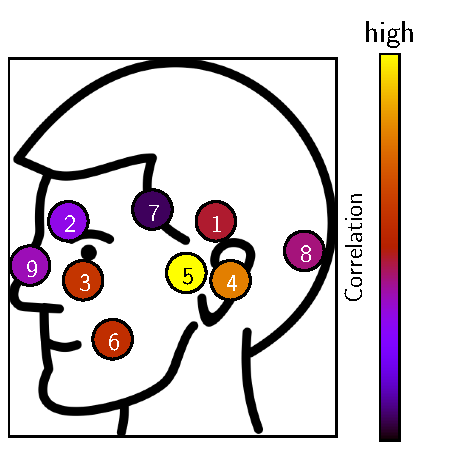
\includegraphics[width=\textwidth]{chapters/vibvoice/figure/correlation.pdf}
    \caption{Intensities of received bone-conducted vibrations on ten locations of the head.}
    \label{fig:vibvoice_head_positison}
\end{minipage}
\hfill
   \begin{minipage}[t]{0.48\columnwidth}
     \centering
    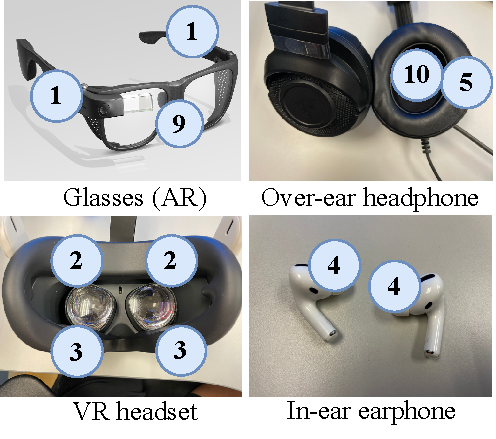
\includegraphics[width=\textwidth]{chapters/vibvoice/figure/devices.pdf}
    \caption{Potential placements on devices.}
    \label{fig:vibvoice_devices}
\end{minipage}
\end{figure}
\noindent\textbf{Locations on the head.}
Bone-conducted vibration exists at various locations on the head. 
As shown in Fig. \ref{fig:vibvoice_head_positison}, we select ten unique locations of interest on the head and measure the intensities of received bone-conducted vibrations. In particular, the nine locations are \#1 \emph{upper ear}, \#2 \emph{eyebrow}, \#3 \emph{cheekbones}, \#4 \emph{ear}, \#5 \emph{temporomandibular joint}, \#6 \emph{cheek}, \#7 \emph{temple}, \#8 \emph{back of the head}, and \#9 \emph{nose}. In addition, we tape EarSense on the interior of the pad of an over-ear headphone, which is denoted as \#10.
Among those positions, some are compatible with commercial HMWs like glasses, headphones, and VR headsets. Fig. \ref{fig:vibvoice_devices} illustrates the corresponding positions on HMWs. The numbers on the HMWs correspond to the locations in Fig. \ref{fig:vibvoice_head_positison}. 
We attach EarSense to the HMWs (when applicable) or on the face for all the following tests. 
We compute Pearson correlation coefficients between the audio and the acceleration on each location and mark the values using a color map in Fig. \ref{fig:vibvoice_head_positison}.
We observe that bone-conducted vibrations exist at most locations of the head. In particular, locations closer to the mouth show higher correlations, indicating a larger possibility of extracting clean speech. 

In summary, our measurements show that bone-conducted vibration has the following characteristics: a) Bone-conducted vibration is robust to environmental voice and only captures the user's speech; b) The user's motion only generates vibrations lower than $85\,\text{Hz}$; c) Bone-conducted vibration has suppressed low and high-frequency audio, which varies across users and within the same user; and d) We can receive audio from multiple locations on the head.


% \section{Motivation Study}
\label{sec:egolog_measurement}
As discussed in Sec. \ref{sec:egolog_intro}, we mainly have three challenges towards a multi-modal HAR on mobile devices: 1) lack of scenario awareness, 2) being sensitive to ambient noise, and 3) fusion collapse. To explore these challenges and evaluate the potential for overcoming them, we conduct a series of experiments to analyze and demonstrate promising directions.

\begin{figure}
    \centering
    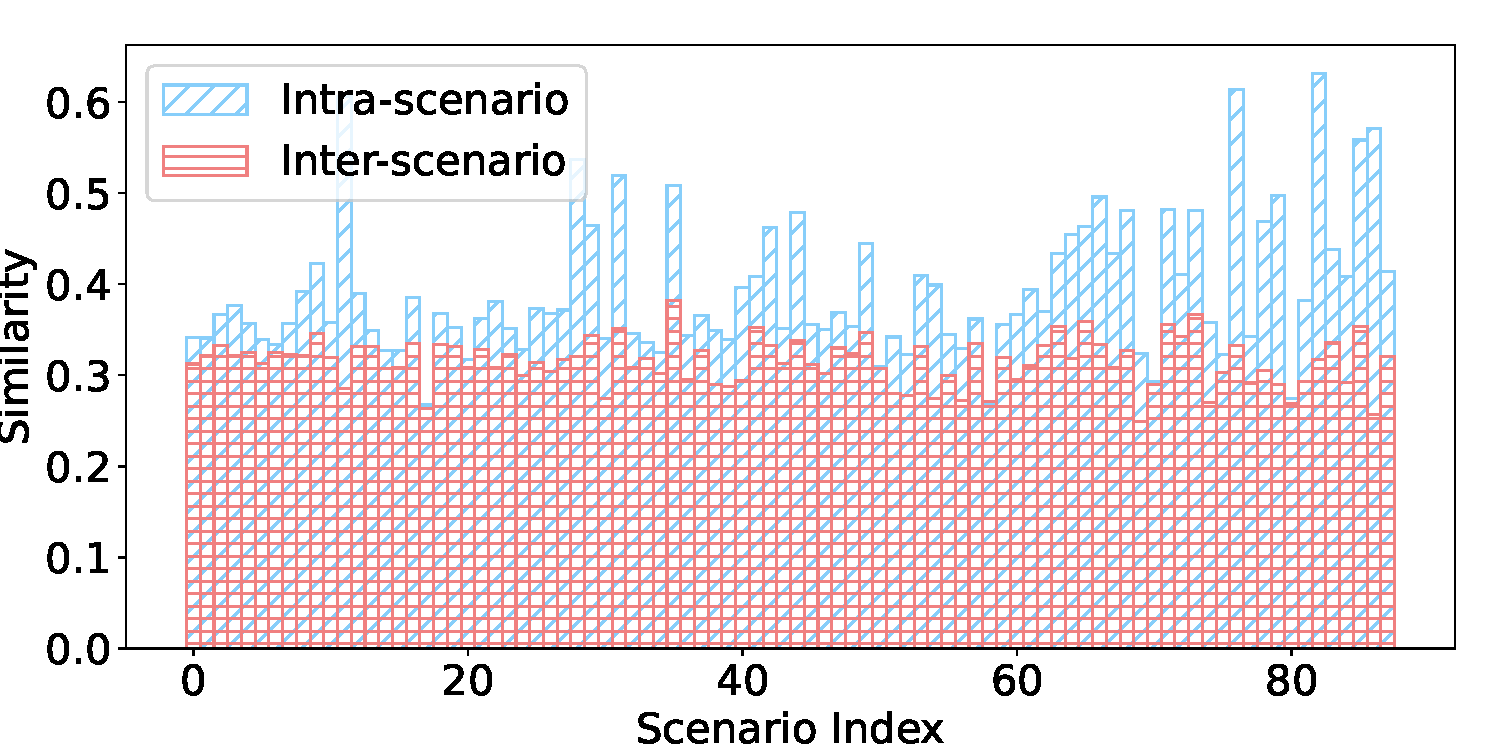
\includegraphics[width=0.8\linewidth]{chapters/egolog/figs/scenario_similarity.pdf}
    \vspace{-1em}
    \caption{Motivation for scenario understanding: 
    The similarity of embeddings for intra- and inter-scenario activities.}
    \label{fig:egolog_scenario_similarity}
    \vspace{-1em}
\end{figure}

\subsection{Scenario}
\label{subsec:scenario}
Scenario information refers to long-time activities (e.g., playing with a pet or working at home) that reflect the user's real-world behavior. Capturing such scenarios in datasets is challenging, as it requires volunteers to perform activities naturally, mimicking real-life conditions. Generally, scenario is the ensemble of multiple related and continuous activities with a realistic distribution, reflecting meaningful interactions with the environment.

To investigate the impact of scenario information on HAR, we use the Ego4D dataset~\citep{grauman2022ego4d}, which captures real-world activities through smart glasses equipped with IMU and audio sensors. The dataset provides annotations at both the window level (every 10 seconds) and the video level, represented as plain text. We treat window-level annotations as activity labels and video-level annotations as scenario labels that describe the broader setting of prolonged activities. To examine scenario properties, we use Sentence-BERT~\citep{reimers2019sentence} to generate text embeddings for activities across 91 scenarios. We then compute activity similarity both within scenarios (intra-scenario) and between scenarios (inter-scenario). Intra-scenario similarity measures the similarity of activities within the same scenario, while inter-scenario similarity compares an activity from one scenario to a randomly selected activity from a different scenario.

The results are shown in Fig.~\ref{fig:egolog_scenario_similarity}, revealing that the similarity within a scenario (intra-scenario similarity) is over 20\% higher than the similarity between different scenarios (inter-scenario similarity). This suggests that each scenario has a distinct distribution of activities. Specifically, a scenario effectively represents the user's daily log since it encompasses a longer time frame.
Additionally, we notice that the inter-scenario similarity is generally above 0.3, indicating that many basic activities (such as sitting and walking) are common across all scenarios. Therefore, it is crucial to eliminate the influence of these basic activities in scenario recognition, as they are present in every scenario.


In summary, the in-the-wild dataset shows that scenarios have distinct activity distributions, which can support scenario recognition through scenario-specific activities.


\subsection{Sound Location }
\label{subsec:embodied}
\begin{figure}
    \centering
    \begin{minipage}{0.48\linewidth}
        \centering
       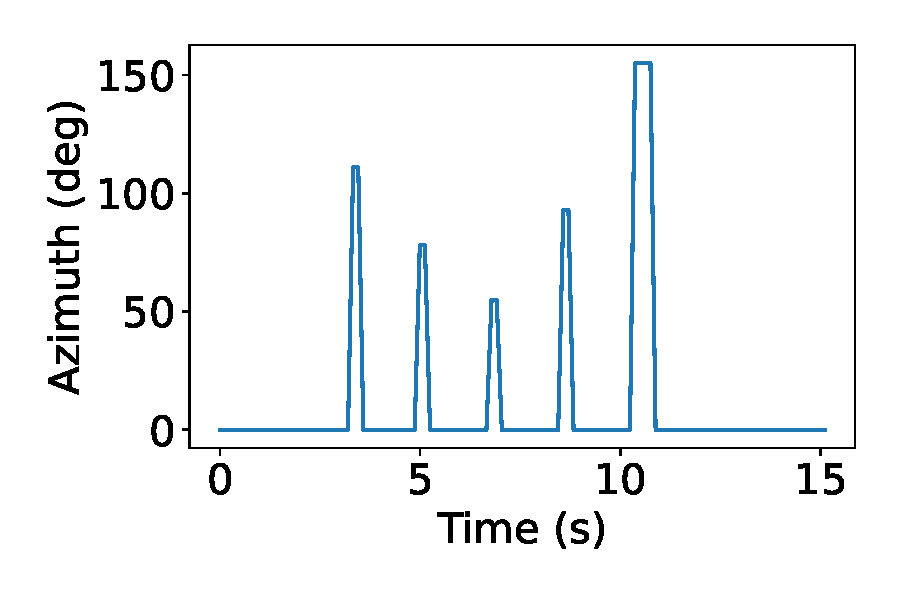
\includegraphics[width=\linewidth]{chapters/egolog/figs/baseline_result.pdf}
        \caption{Sound localization \citep{schmidt1986multiple} under motion}
        \label{fig:egolog_loc_move}
    \end{minipage}
    \hfill
    \begin{minipage}{0.48\linewidth}
        \centering
        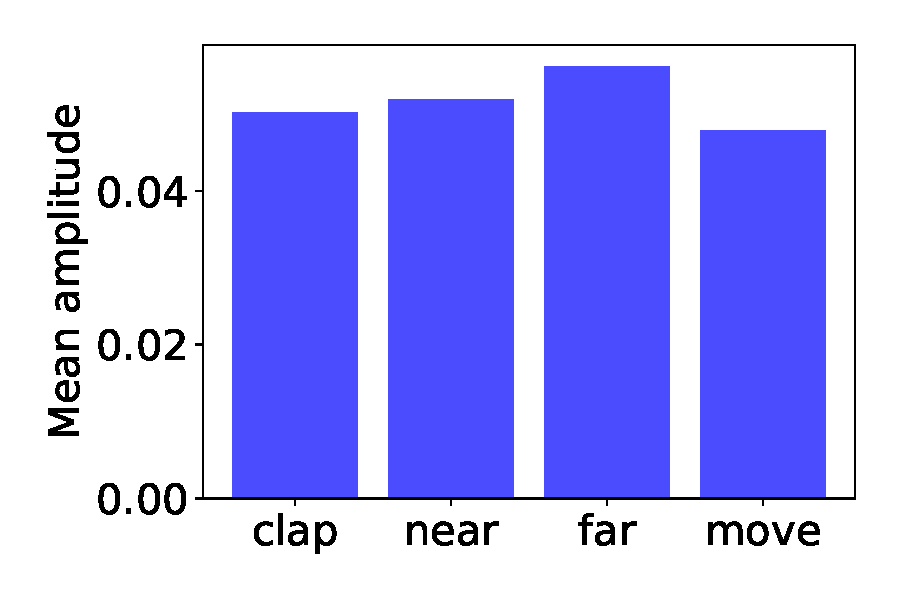
\includegraphics[width=\linewidth]{chapters/egolog/figs/amplitude.pdf}
        \caption{Sound volume may not related to distance.}
        \label{fig:egolog_amplitude}
    \end{minipage}    
    \vspace{-1em}
\end{figure}

\begin{figure}
    \centering
    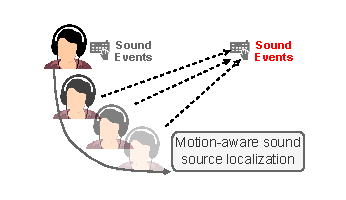
\includegraphics[width=0.75\linewidth]{chapters/egolog/figs/spatial_motivation.pdf}
    \vspace{-1em}
    \caption{Motivation for spatial understanding: estimate the distance of a sound event by motion.}
    \vspace{-1em}
    \label{fig:egolog_motivation_localization}
\end{figure}

In practice, recorded audio often includes far-field sound sources that are unrelated to the user’s activities, underscoring the importance of sound localization for effective HAR. Wearables that are consistently worn on the user’s head provide a stable and reliable position for capturing detailed ambient sound information. Additionally, modern wearables feature multi-channel recording capabilities, enhancing their spatial sensing potential.
In the following, we divide sound localization into direction and distance estimation, which we discuss as follows.

The estimation of sound direction is one of the mature, basic, but still challenging applications of a microphone array. The accuracy highly depends on the number of microphones, which is unfortunately not sufficient for most commercial devices. Considering the most common setting of stereo recording, there are mainly two problems: the deviation of direction (especially for front-back confusion) and estimation of sound distance, as illustrated in Fig. \ref{fig:egolog_motivation_localization}.
We envision that the above challenges may be solved by motion compensation. Specifically, we can aggregate the consecutive sound localization results along with the movement of the user (microphone) to refine the results or even get the distance.

To illustrate these challenges, we positioned a sound source in front of the user and used a binaural microphone with the algorithm from~\citep{schmidt1986multiple} to estimate direction of arrival, as shown in Fig.~\ref{fig:egolog_loc_move}. The user was instructed to move the body slightly and naturally. The estimate fluctuated around the true value of 90 degrees. To test whether sound volume is sufficient for differentiating near and far sources, we conducted an experiment with the sound source at different distances from the microphone. As shown in Fig.~\ref{fig:egolog_amplitude}, volume differences were not reliable across distances. The final bar in Fig.~\ref{fig:egolog_amplitude} also shows that user movement slightly affects amplitude. Multiple sound sources can further complicate volume-based distance estimation.

\subsection{Multi-modal Fusion }
\label{subsec:measure-fuse}

\begin{figure}
    \centering
     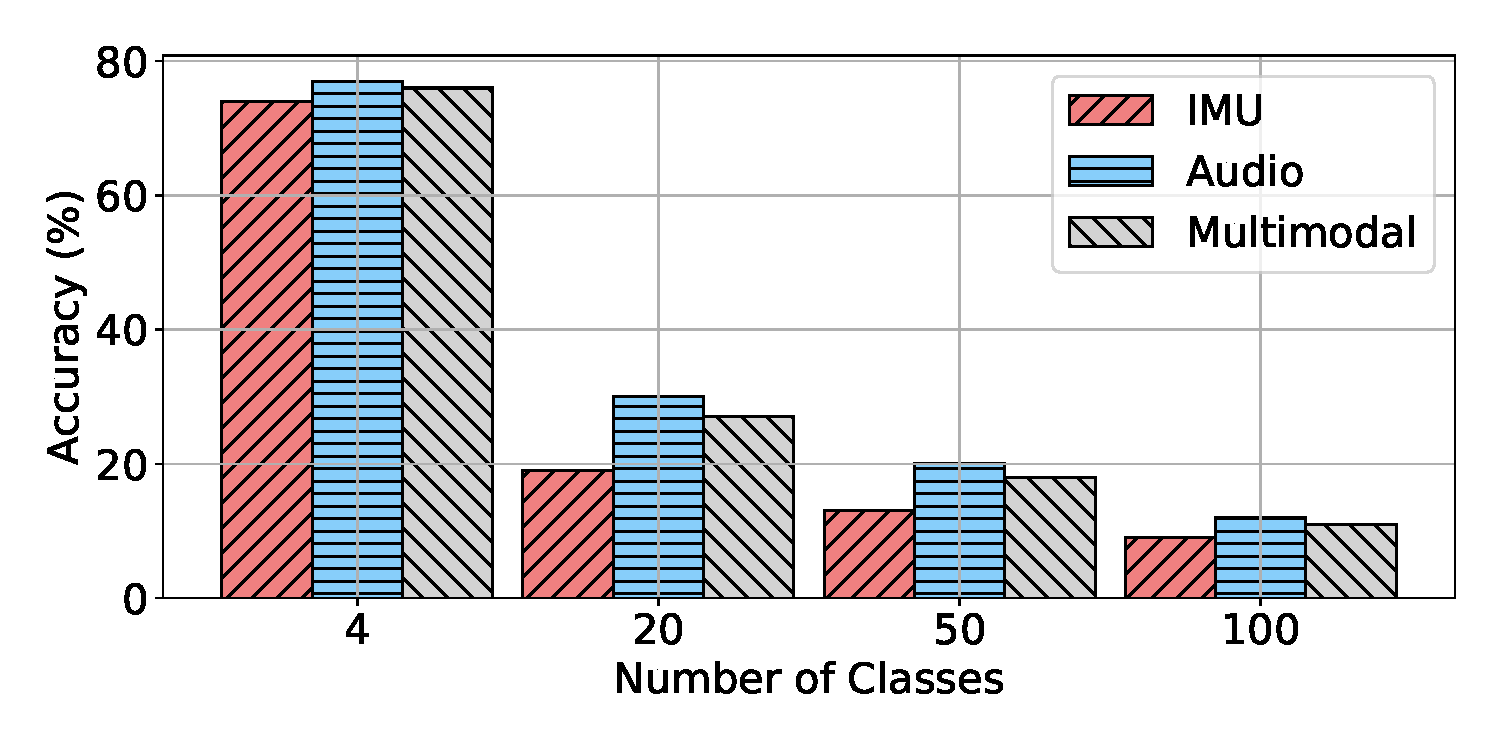
\includegraphics[width=.75\linewidth]{chapters/egolog/figs/num_class.pdf}
     \vspace{-1em}
      \caption{The performance of an existing activity recognition with different class numbers and modalities.}
    \label{fig:egolog_num_class}
    \vspace{-1em}
\end{figure}

To investigate scalability bottlenecks in activity recognition using wearables, we trained unimodal supervised models with audio and IMU data on the Ego4D episodic memory subset (200 activity classes). We used EfficientAT~\citep{schmid2023efficient} for audio and LIMU-BERT~\citep{xu2021limu} for IMU as feature extraction backbones, comparing them to a multi-modal model via late fusion. Activities were clustered into varying class numbers using Sentence BERT~\citep{reimers2019sentence} embeddings and K-Means~\citep{macqueen1967some}, following MMG-Ego4D~\citep{gong2023mmg}. Results (Fig.~\ref{fig:egolog_num_class}) show a significant performance drop as class numbers increase, indicating challenges in recognizing diverse activities with audio or IMU alone. Multimodal fusion often underperforms unimodal models, suggesting ineffective extraction of complementary features at larger scales.

\begin{figure}
    \centering
    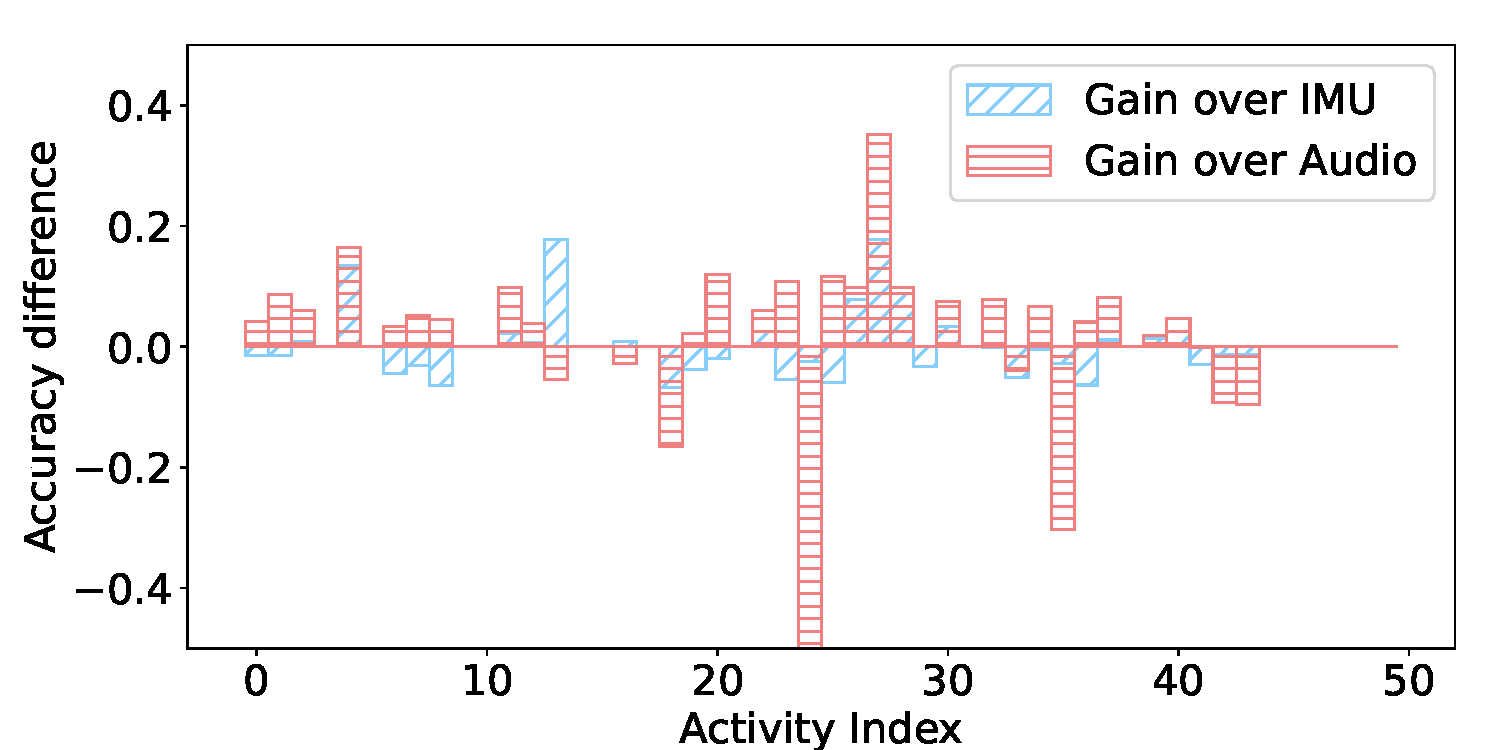
\includegraphics[width=.75\linewidth]{chapters/egolog/figs/activity_diff.pdf}
    \vspace{-1em}
    \caption{Performance gain from multi-modal fusion.}
    \label{fig:egolog_acc_gap}
    \vspace{-1em}
\end{figure}

Previous work~\citep{mollyn2022samosa} demonstrates that multi-modal learning can outperform the unimodal model due to the complementary nature of each other.
However, this finding does not apply to all cases. Another study~\citep{gong2023mmg} finds that multimodal learning with audio and IMU on Ego4D can perform worse than single-modality solutions. To investigate this result, we compared the accuracy of multimodal and unimodal models for each class, as shown in Fig.~\ref{fig:egolog_acc_gap}. The benefits of multimodal fusion fluctuate across both modalities, indicating that supervised multimodal learning cannot automatically select the appropriate modality for each activity.


To investigate whether LLMs can alleviate this problem, we evaluate ImageBind-LLM~\citep{han2023imagebind}, which converts both modalities into features and prepends them to text embeddings. We instruct the model with the prompt: ``<sensor> According to the audio and IMU reading on the earphone of the user, what is the activity of the user?'', where <sensor> denotes the inserted sensor features. Since LLM outputs can be random, we also constrain the prompt to one of the candidate activities. To reduce complexity, we select the top 30 activities from the Ego4D episodic memory subset. ImageBind-LLM achieves BERT-score precision, recall, and F1 score of 0.04, 0.07, and 0.05, respectively. Because this performance is low, we inspect the outputs and find that the LLM may not fully understand the multimodal fusion task.
We further test whether fine-tuning can address this problem by training an adapter~\citep{zhang2023llamaadapter} for ImageBind-LLM. The adapted LLM achieves BERT-score precision, recall, and F1 score of 0.47, 0.46, and 0.47, respectively. Although fine-tuning improves performance, the result remains below the level needed for practical use.

% \section{Background}
\label{sec:cohear_background}

This section lays the technical foundation for CoHear, focusing on acoustic sensing techniques used for conversation modeling.
First, it discusses sound localization, which estimates speaker positions from earphone microphone arrays and provides information for constructing a conversation map.
It then reviews wireless acoustic sensor networks (WASNs), which support collaborative sensing across multiple devices.


\subsection{Sound Source Localization}
Sound source localization is a core problem in multi-channel audio and enables spatial acoustic sensing.
Consider a microphone array consisting of $N$ microphones located at known positions $\mathbf{p}_i = (x_i, y_i)$ for $i = 1, 2, \ldots, N$. Let the position of the sound source be denoted by $\mathbf{s} = (x_s, y_s)$.
The time it takes for the sound to reach the microphone $i$ can be expressed as:
\(t_{s, i} = \frac{d_{s, i}}{c}, d_{s, i} = \sqrt{(x_s - x_i)^2 + (y_s - y_i)^2}\)
where $d_{s, i}$ is the distance from sound source $s$ to microphone $i$, and $c$ is the speed of sound in air. Since the source emission time is unknown to the receiver, $t_{s, i}$ cannot be estimated directly. Instead, the system estimates the time difference of arrival (TDoA), $t_{s, i} - t_{s, j}$, where $i, j \in (1, N)$. A common method for estimating TDoA from in-the-wild recordings is the generalized cross-correlation (GCC)~\cite{knapp1976generalized}, which is computed for each microphone pair. The GCC peak estimates the TDoA, which can then be used to calculate the direction of arrival (DoA) as \(DoA = arctan((x_s - x_c)/(y_s - y_c))\), where $x_c$ is the center of the microphone array. This analysis shows why localization performance depends strongly on the number of microphones: more microphones provide more microphone pairs and therefore more TDoA constraints.

Instead of relying on analytical methods, sound source localization can be performed using a deep neural network, as explored in \cite{wang2022nerc}. This deep learning-based approach generally consists of two stages: feature extraction and location estimation.
In the feature extraction stage, the audio signal is typically converted into a spectrogram representation with dimensions: \(C\times T \times F\), where \(C\) refers to channels, \(T\) refers to time, and \(F\) refers to frequency. These features can be further processed using techniques such as log-melspectrogram conversion, which is applied to each channel individually, or multi-channel methods like GCC \cite{knapp1976generalized} and SALSA-Lite \cite{nguyen2022salsa}.
In the location estimation stage, the neural network is trained to output the sound source location, which also supports a dynamic number of simultaneous sound sources. For instance, architectures employing multi-track \cite{cao2021improved} or multi-ACCDOA \cite{shimada2022multi} output formats are designed specifically to localize overlapping sound events.

Deep sound localization can also use the spatial information embedded in binaural recordings, including reflections from the human head and body. Specifically, the head-related transfer function (HRTF) can be modeled as:
\(H_{L}(\theta, \phi, f, d) = \frac{Y_{L}(f)}{X(f)}, H_{R}(\theta, \phi, f, d) = \frac{Y_{R}(f)}{X(f)},\) where $H_{L}$ indicates the frequency response for left ear and $H_{R}$ indicates the frequency response for right ear. 
By using HRTF cues with deep learning, binaural localization can achieve higher accuracy than a linear two-microphone array. For instance, this approach can partially resolve front--back confusion, a problem that is particularly challenging for conventional two-microphone arrays.


\subsection{Wireless Acoustic Sensor Network}
We are studying a wireless acoustic sensor network where a group of sensor nodes is randomly distributed in a reverberant environment \cite{bertrand2011applications}. We assume that the internal geometric configuration of each node's microphone array is known and that all microphones within the array are sampled at the same time, which we believe is a reasonable assumption following \cite{gburrek2021geometry}. Additionally, we assume that there is coarse time synchronization among the clocks of the sensor nodes, enabling us to aggregate the data globally. By default, we assume a two-dimensional space, but it can be easily extended to a three-dimensional space.

Since a sensor node cannot determine its own position or orientation within the global coordinate system, all observations are made in the local coordinate system of each node. 
Each sensor node \( l \) (where \( l = 1, \ldots, L \)) computes acoustic features (e.g., DoA estimates \( \phi_k^l \) and distance \( d_k^l \)) to the acoustic source \( k \), all reference to the node's local coordinate system. Consequently, we gather a total of \( K \times L \) estimates as the inputs.

From the global view of the WASN, it is composed of \( L \) sensor nodes each equipped with a microphone array located at positions \( n_l = [n_{l,x}, n_{l,y}]^T \) and oriented at angles \( \theta_l \) (where \( l = 1, 2, \ldots, L \)) relative to a global coordinate system defined by the x and y axes. There are \( K \) acoustic sources located at positions \( s_k = [s_{k,x}, s_{k,y}]^T \) (where \( k = 1, 2, \ldots, K \)). Note that all the above global notations are unknown and will be estimated through a geometry calibration process based on the observed acoustic signals from sensor nodes.





This chapter outlines the principles of user–environment sensing using head-mounted wearables, focusing on topics within the scope of this thesis.
We first discuss the available sensing modalities, their properties, and limitations.
We then introduce the core algorithms that enable sensing with these modalities.
Lastly, we present measurement studies that substantiate and elaborate on the above discussions.

\section{Sensors on Head-mounted Wearables}
Modern head-mounted wearables are typically equipped with multiple sensors to capture various aspects of the user's environment and activities, including, but not limited to, microphones that capture audio, inertial measurement units (IMUs) that capture motion and orientation, and cameras that capture visual information. We discuss these in the following subsections.

\subsection{Microphone}
A microphone (mic) converts fluctuations in air pressure into an electrical signal. It is fundamental to telecommunication, audio capture, broadcasting, and many consumer devices, including phones, hearing aids, and head-mounted wearables. Common transduction mechanisms include dynamic moving-coil elements operating in a magnetic field, condenser (capacitor) capsules where a tensioned diaphragm forms one plate, and contact/piezo designs that exploit piezoelectric crystals. Because microphone outputs are low level, they are typically routed through a preamplifier before recording or playback.

Due to the compact form factor of head-mounted wearables, the microphones used in these devices are typically small and lightweight, which generally implies fewer microphones, a narrower frequency response, and lower sensitivity compared to professional-grade equipment.
Importantly, they are often omnidirectional, which offers broad applicability but also captures more ambient noise.

In head-mounted wearables, microphones are the primary means of capturing the user's voice and ambient sound.

\subsection{Inertial Measurement Unit}
Inertial Measurement Units (IMUs) are electronic devices that measure and report a body's specific force, angular rate, and sometimes the magnetic field surrounding the body, using a combination of accelerometers, gyroscopes, and optionally magnetometers. The traditional application of IMUs is tracking the orientation and movement of objects, such as in aerospace, robotics, and consumer electronics like wearables.

Combining IMUs with other sensors, such as cameras or Global Positioning System (GPS), provides more accurate and robust motion tracking and navigation capabilities, addressing challenges such as error accumulation in IMU-only systems.

IMUs are now used beyond tracking. In particular, they are key sensors for activity recognition by analyzing complex patterns in the IMU readings. IMUs are ubiquitous, low-power, and privacy-preserving—key advantages over many other sensors. Major applications include step counting, gait analysis, sports recognition, gesture recognition, and fall detection.

\subsection{Cameras}
Cameras are optical devices that capture visual information by recording light patterns onto a photosensitive surface or digital sensor. They are widely available on head-mounted wearables, especially high-end devices like AR/VR headsets and smart glasses. 

The applications of cameras on head-mounted wearables are diverse, ranging from recognizing the user (e.g., expression, eye movement, hand movement) to sensing the surrounding environment (e.g., object tracking).
Although cameras are powerful, they also bring significant challenges in terms of privacy, power consumption, and data processing requirements.
Within the scope of this thesis, we mainly focus on applications that do not assume cameras, making the methods applicable to more general head-mounted wearables. Integration of camera data can, of course, further enhance system performance.

\subsection{Speaker}
A speaker is an electroacoustic transducer that converts an electrical audio signal into corresponding sound—the reverse of a microphone.
Speakers are designed for audio output (communication, media playback, notifications), not sensing. However, researchers have discovered that speakers can also be used as sensors in certain scenarios. For example, by analyzing reflected sound waves emitted by a speaker, it is possible to infer information about the surrounding environment, such as distance to objects or movement patterns—similar to sonar or echolocation. This principle is applicable to head-mounted wearables with built-in speakers.

\subsection{Biometric Sensor}
Due to the proximity of head-mounted wearables to the skin and the head, they can also incorporate biometric sensors to monitor physiological signals. Common biometric sensors include photoplethysmography (PPG) sensors for heart rate monitoring, which can be embedded within earbud tips. Or, temperature sensors for skin temperature measurement. Except for the specific sensors of biometric, sensors like microphone and IMU can also be used for biometric purposes, e.g., using microphone for heartbeat detection via the ear-canal listening.

\section{Algorithms}
This section introduces the fundamental algorithms that enable user–environment sensing using the sensors on head-mounted wearables, within the scope of this thesis.

\subsection{Sound Enhancement and Separation}
Suppose the audio recorded by the microphone on head-mounted wearables is denoted as \(y(t)\), which is a mixture of the target sound \(s(t)\) and undesired noise \(n(t)\): \[y(t) = s(t) + n(t).\] A sound enhancement or separation algorithm aims to recover the target sound \(s(t)\) from the mixture \(y(t)\) by a model \(f(\cdot)\): \[\hat{s}(t) = f(y(t)),\] where \(\hat{s}(t)\) is the estimated target sound.

Notably, the "target" is scenario-dependent rather than fixed. For example, in speech enhancement the target is clean speech, whereas in music separation the target could be a specific instrument or vocal track. We therefore use the general term "sound enhancement and separation" to cover both tasks.

To achieve separation, one may use either traditional signal processing techniques or modern deep learning-based methods. Traditional techniques include spectral subtraction, Wiener filtering, and beamforming, which rely on statistical properties of noise so that the algorithm can filter out similar components: \[ \hat{s}(t) = f(y(t), n_{\text{ref}}(t)).\]
With the advancement of deep learning, data-driven approaches have become increasingly popular and often achieve superior performance.
Generally, deep learning models do not rely on explicit assumptions about noise characteristics; instead, they learn to distinguish target from noise using large datasets: \[ \hat{s}(t) = f_{\theta}(y(t)).\] Although large datasets confer strong generalization capability, models may still lack adaptability to unseen noise types and acoustic conditions.

Recently, target sound extraction has been proposed to further improve performance, where an additional reference signal \(s_{\mathrm{ref}}(t)\) is provided to guide the model to focus on the desired target: \[ \hat{s}(t) = f_{\theta}\big(y(t), E\big(s_{\mathrm{ref}}(t)\big)\big),\] where \(E\) is an encoder that extracts target characteristics from the reference signal (which can be any signal related to the target sound). This paradigm is a form of multi-modal learning, where the model leverages information from multiple modalities to enhance performance. 

\subsection{Multi-channel Audio Processing}
\label{sec:cohear_background}

This section lays the technical foundation for multi-channel audio processing, which is essential for the design in \ref{ch:cohear}. The basic assumption is that more than one microphone is available for audio recording, which differs from single-microphone processing.
First, we discuss sound localization, which identifies speaker positions using earphone microphone arrays, providing essential information to create a conversation map.
Next, we review Wireless Acoustic Sensor Networks (WASNs), which facilitate collaborative sensing across multiple devices.

\subsubsection{Sound Source Localization}
Sound source localization is one of the hot topics for multi-channel audio, which enables spatial sensing capability for audio.
Consider a microphone array consisting of $N$ microphones located at known positions $\mathbf{p}_i = (x_i, y_i)$ for $i = 1, 2, \ldots, N$. Let the position of the sound source be denoted by $\mathbf{s} = (x_s, y_s)$.
The time it takes for the sound to reach the microphone $i$ can be expressed as:
\(t_{s, i} = \frac{d_{s, i}}{c}, d_{s, i} = \sqrt{(x_s - x_i)^2 + (y_s - y_i)^2}\)
where $d_{s, i}$ is the distance from the sound source $s$ to microphone $i$, and $c$ is the speed of sound in air. Since the sound source is unknown to the receiver, we cannot directly estimate $t_{s, i}$ but calculate the time difference of arrival (TDoA) $t_{s, i} - t_{s, j}$, where $i, j \in \{1, \ldots, N\}$. To estimate TDoA from in-the-wild recordings, a common approach is Generalized Cross-Correlation (GCC) \cite{knapp1976generalized}, computed for each pair of microphones. By finding the GCC peak, we estimate TDoA and calculate the direction of arrival (DoA) by \(\mathrm{DoA} = \arctan\big((x_s - x_c)/(y_s - y_c)\big)\), where $x_c$ refers to the center of the microphone array. As shown above, sound localization performance relies heavily on the number of microphones (more microphones yield more pairs and thus more TDoA estimates). 

Instead of relying on analytical methods, sound source localization can be performed using a deep neural network, as explored in \cite{wang2022nerc}. This deep learning-based approach generally consists of two stages: feature extraction and location estimation.
In the feature extraction stage, the audio signal is typically converted into a spectrogram representation with dimensions: \(C\times T \times F\), where \(C\) refers to channels, \(T\) refers to time, and \(F\) refers to frequency. These features can be further processed using techniques such as log-melspectrogram conversion, which is applied to each channel individually, or multi-channel methods like GCC \cite{knapp1976generalized} and SALSA-Lite \cite{nguyen2022salsa}.
In the location estimation stage, the neural network is trained to output the sound source location, which also supports a dynamic number of simultaneous sound sources. For instance, architectures employing multi-track \cite{cao2021improved} or multi-ACCDOA \cite{shimada2022multi} output formats are designed specifically to localize overlapping sound events.

Besides, deep sound localization can extract the rich information embedded in binaural recording (microphones on the ears), which comprises the complex reflection from the human head and body. Specifically, the head-related transfer function (HRTF) can be modeled as:
\(H_{L}(\theta, \phi, f, d) = \frac{Y_{L}(f)}{X(f)}, H_{R}(\theta, \phi, f, d) = \frac{Y_{R}(f)}{X(f)},\) where $H_{L}$ indicates the frequency response for left ear and $H_{R}$ indicates the frequency response for right ear. 
By leveraging HRTF and deep learning, we can achieve higher accuracy than using a linear two-microphone array. For instance, this approach can partially resolve front-back confusion, a problem that is particularly challenging for conventional two-microphone arrays.

\subsubsection{Wireless Acoustic Sensor Network}
We are studying a wireless acoustic sensor network where a group of sensor nodes is randomly distributed in a reverberant environment \cite{bertrand2011applications}. We assume that the internal geometric configuration of each node's microphone array is known and that all microphones within the array are sampled at the same time, which we believe is a reasonable assumption following \cite{gburrek2021geometry}. Additionally, we assume that there is coarse time synchronization among the clocks of the sensor nodes, enabling us to aggregate the data globally. By default, we assume a two-dimensional space, but it can be easily extended to a three-dimensional space.

Since a sensor node cannot determine its own position or orientation within the global coordinate system, all observations are made in the local coordinate system of each node. 
Each sensor node \( l \) (where \( l = 1, \ldots, L \)) computes acoustic features (e.g., DoA estimates \( \phi_k^l \) and distance \( d_k^l \)) to the acoustic source \( k \), all reference to the node's local coordinate system. Consequently, we gather a total of \( K \times L \) estimates as the inputs.

From the global view of the WASN, it is composed of \( L \) sensor nodes each equipped with a microphone array located at positions \( n_l = [n_{l,x}, n_{l,y}]^T \) and oriented at angles \( \theta_l \) (where \( l = 1, 2, \ldots, L \)) relative to a global coordinate system defined by the x and y axes. There are \( K \) acoustic sources located at positions \( s_k = [s_{k,x}, s_{k,y}]^T \) (where \( k = 1, 2, \ldots, K \)). Note that all the above global notations are unknown and will be estimated through a geometry calibration process based on the observed acoustic signals from sensor nodes.

\subsection{Human Activity Recognition}
The application of IMU sensors for human activity recognition (HAR) represents a paradigm shift from their original motion tracking purpose. Rather than precisely reconstructing trajectories—which requires sophisticated tracking algorithms such as Kalman filters—HAR focuses on identifying characteristic motion patterns associated with specific activities.

Consider step counting as an illustrative example. Traditional motion tracking would compute the sensor's horizontal displacement over time, accumulating position estimates that are prone to drift. In contrast, HAR-based step counting disregards absolute position entirely, instead detecting the periodic acceleration patterns generated by each footstep. Formally, IMU data is represented as a \( 6 \times T \) matrix, where the six channels correspond to three-axis accelerometer and three-axis gyroscope readings, and \( T \) denotes the number of time steps. Traditional step counting algorithms analyze the vertical acceleration channel to identify periodic peaks corresponding to foot strikes. However, this rule-based design does not generalize to more complex activities such as running, jumping, or cycling. Although these activities exhibit distinctive motion patterns, the differences cannot be adequately captured by a small set of handcrafted rules.

To address this limitation, modern HAR systems predominantly employ deep learning methods that treat IMU data as a two-dimensional input, typically following a two-stage pipeline: feature extraction followed by activity classification. Despite recent advances, most models remain relatively simple architectures, primarily due to the scarcity of large-scale, diverse HAR datasets. With the emergence of larger datasets and advances in large language models, the capability of HAR systems is being extended toward more complex and broader real-world scenarios.

\section{Measurement Study}

\subsection{Speech Enhancement}
\label{sec:vibvoice_background}
In this section, we first introduce EarSense, an open-source wearable platform with a setup similar to current commercial HMWs for data collection (Section \ref{sec:vibvoice_EarSense}). We then analyze bone-conducted vibrations and audio signals recorded by EarSense under various settings (Section \ref{sec:vibvoice_measurement}). Finally, we overview our proposed system (Section \ref{sec:vibvoice_overview}) and introduce the Bone Conduction Function and a multi-modal network (Sections \ref{sec:vibvoice_bcf} and \ref{sec:vibvoice_network}).


\subsubsection{EarSense: An Open Source Data Collection Platform for HMWs}
\label{sec:vibvoice_EarSense}

Most commercial HMWs do not provide APIs to collect raw acceleration data. Recently, Apple provided APIs \citep{CMHeadph3:online} to collect motion data from AirPods earphones at $100\,\text{Hz}$, which is too low for speech recording and does not fully utilize commercial IMUs.
Hence, it is desirable to develop a new sensing platform that can: a) collect acceleration and acoustic data synchronously at a sampling rate sufficient to recover speech information; b) have direct contact with the user's head like HMWs; and c) remain compatible for testing with existing commercial devices.
\begin{figure}
  \begin{subfigure}{.64\columnwidth}
    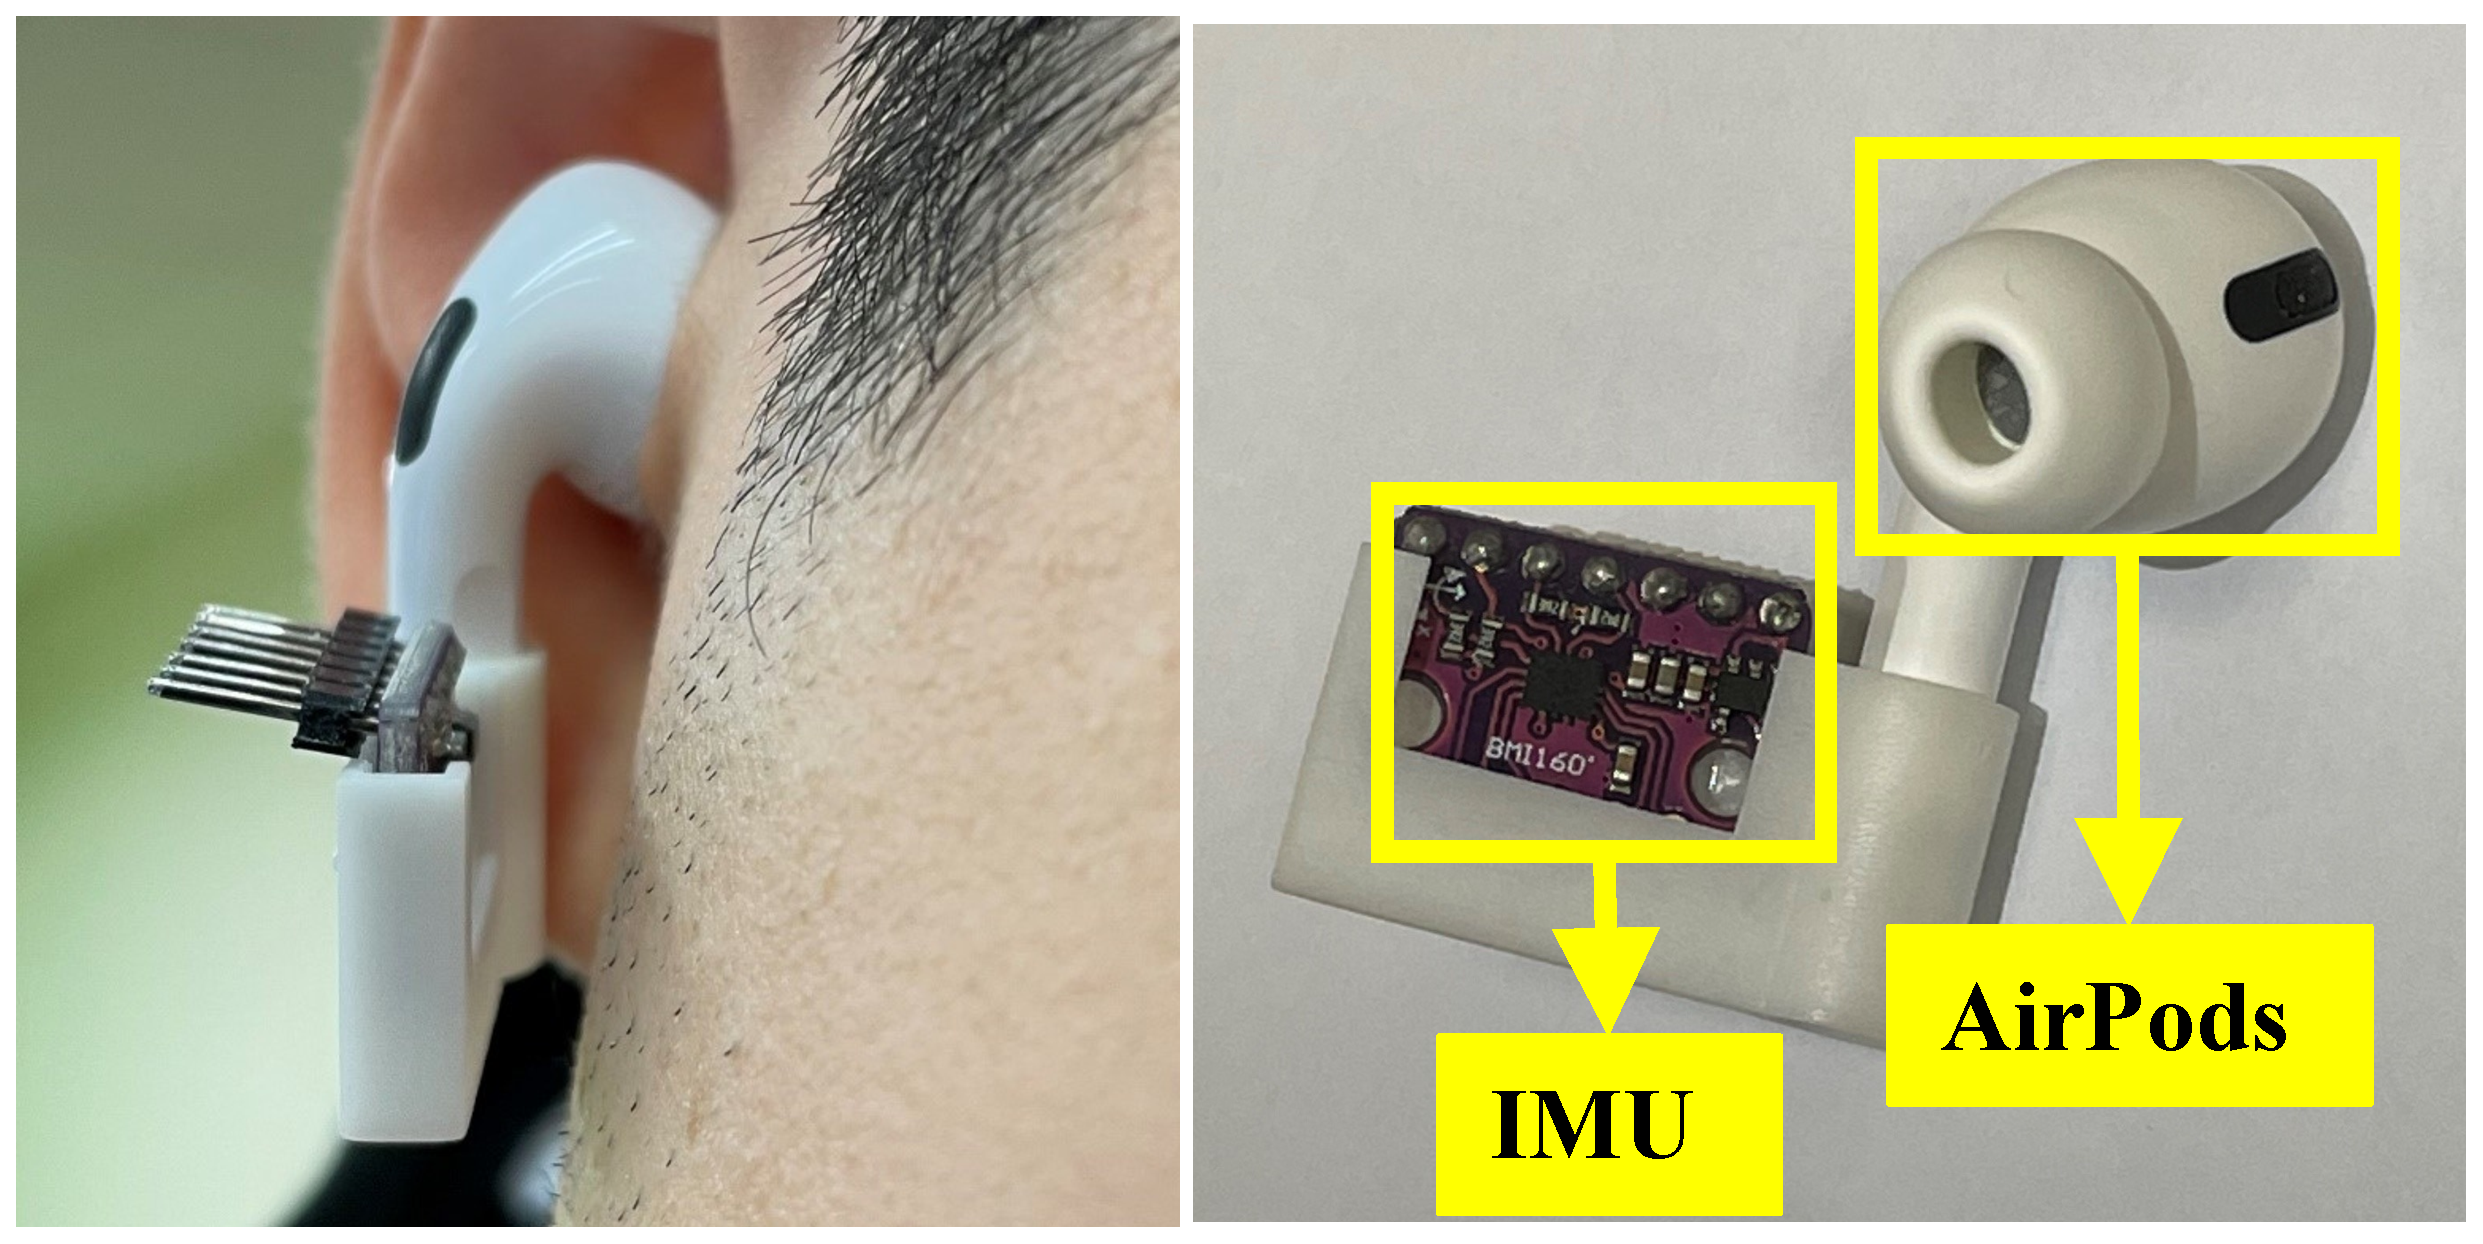
\includegraphics[width=\textwidth]{chapters/vibvoice/figure/earsense.eps}
    \caption{\emph{EarSense} with an Airpods Pro.}
    \label{fig:vibvoice_earsense-head}
  \end{subfigure}
  \begin{subfigure}{0.35\columnwidth}
    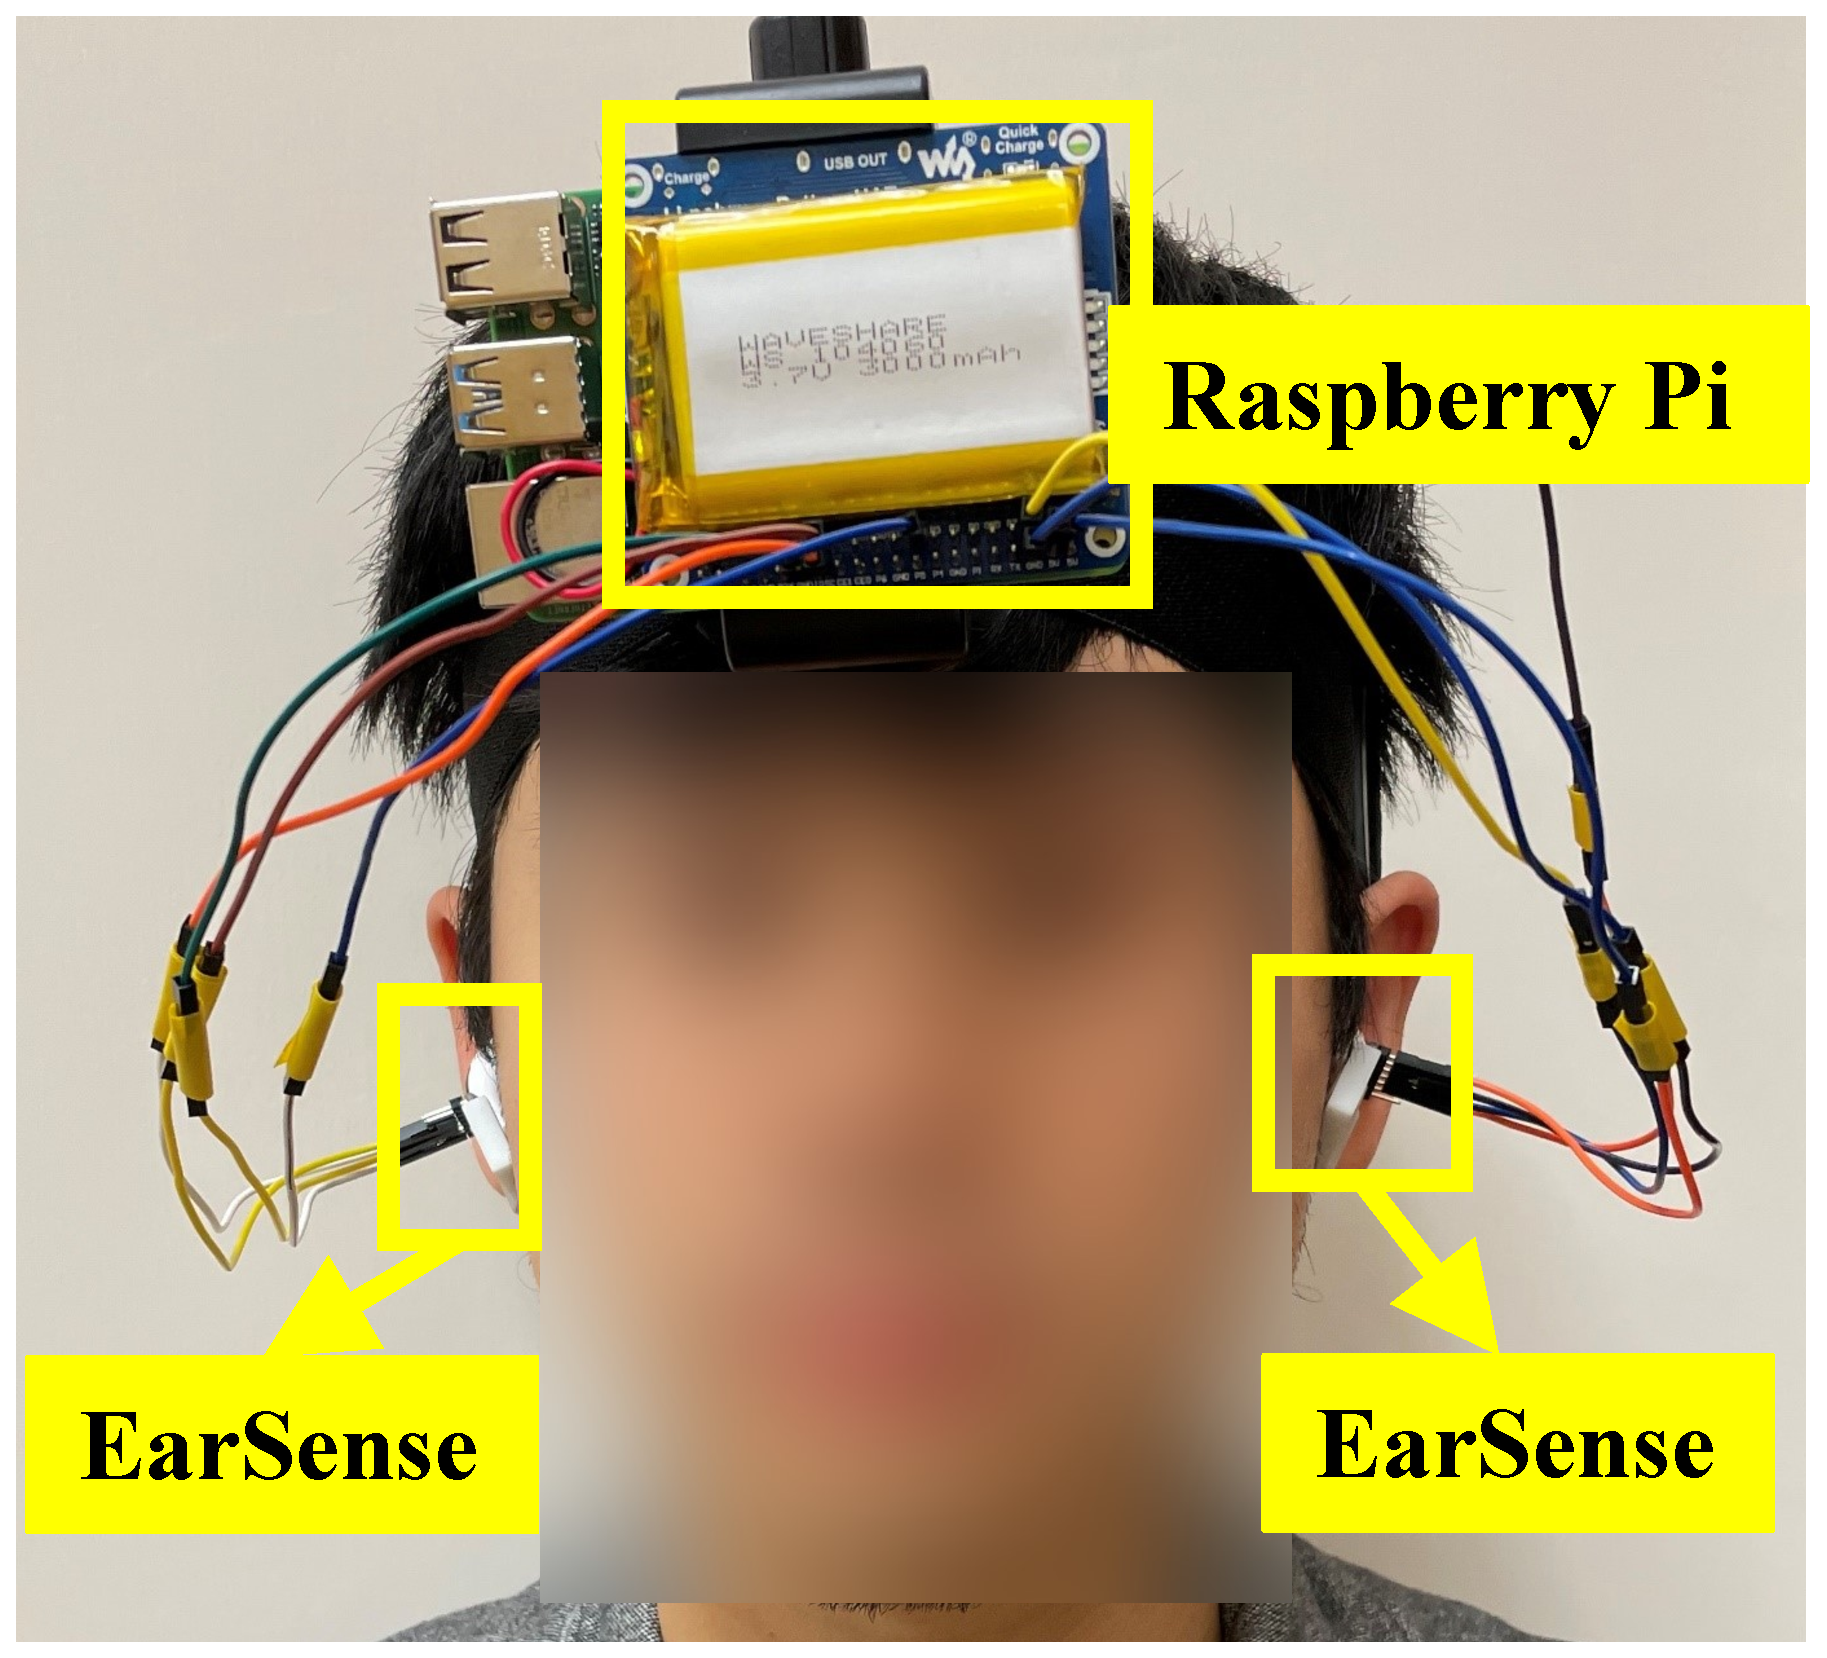
\includegraphics[width=\textwidth]{chapters/vibvoice/figure/people.eps}
    \caption{Test Setup.}
    \label{fig:vibvoice_earsense-people}
  \end{subfigure}
  \caption{\emph{EarSense} is an open-sourced data collector attachable to commercial HMWs for vibration sensing.}
  \label{fig:vibvoice_earsense}
\end{figure}

Fig. \ref{fig:vibvoice_earsense} shows the prototype of \textit{EarSense} \citep{dataset}, a new open-sourced sensing platform that houses an IMU sensor (Bosch BMI-160 \citep{Inertial63:online}) in a 3D-printed enclosure. EarSense has a flexible design that makes it attachable to commercial HMW devices (e.g., AirPods Pro). EarSense captures the same vibrations as the tested HMW and has no direct contact with the user's head (Fig. \ref{fig:vibvoice_earsense-head}).
We connect two EarSenses to a Raspberry Pi (RPi) with a battery for data collection.
Fig. \ref{fig:vibvoice_earsense-people} shows a volunteer wearing the device on the head to avoid excessive vibrations caused by the connecting wires.
A Python script on the RPi controls the EarSense(s) through the I2C protocol and stores the data for offline processing.
We use only the three-axis accelerometer provided by the IMU chip because the gyroscope and magnetometer are less related to the vibration.
The default sampling rates of the microphone and the accelerometer are $16\,\text{kHz}$ and $1.6\,\text{kHz}$, respectively. Since commercial earphones like AirPods Pro do not support two-channel audio recording, EarSense records audio in a mono channel.
We apply the L2 norm to the spectrograms of three-axis acceleration to extract vibration intensity and avoid the impact of wearing position and user motion.

\subsubsection{Measurements of Bone-Conducted Vibrations}
\label{sec:vibvoice_measurement}
We measure the differences between audio and bone-conducted vibrations with EarSense under various settings—specifically, competing speakers and user motion. In each experiment, we ask a volunteer to wear Apple AirPods Pro with EarSense attached (Fig. \ref{fig:vibvoice_earsense-people}) in a meeting room of size $10~\text{m}^2$. 
\begin{figure}
    \begin{subfigure}{0.46\columnwidth}
        \centering
        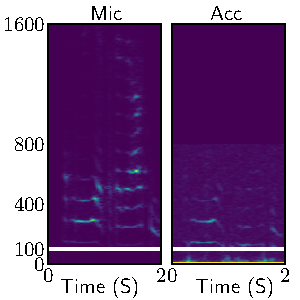
\includegraphics[width=1\textwidth]{chapters/vibvoice/figure/clean.pdf}
        \caption{The user is talking with no noise.}
        \label{fig:vibvoice_nospeaker}
        \end{subfigure}
        \hspace{.5em}
    \begin{subfigure}{0.46\columnwidth}
        \centering
        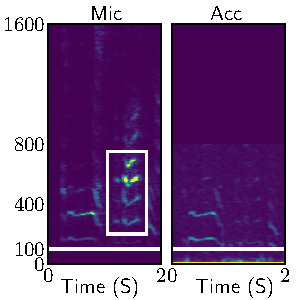
\includegraphics[width=1\textwidth]{chapters/vibvoice/figure/noise.pdf}
        \caption{The user is talking with a competing speaker.}
        \label{fig:vibvoice_speaker}
         \end{subfigure}
    \caption{Impact of the competing speaker.}
    \label{fig:vibvoice_competing-speaker}
\end{figure}

\noindent\textbf{Competing speaker.}
First, we ask the user to sit in the meeting room and speak while a loudspeaker plays pre-recorded speech one meter from the user as the competing speaker. Competing speakers are among the most challenging environmental noises for HMWs because their spectra resemble speech, making them difficult for noise suppression algorithms.
We set the competing speaker's volume similar to the user's, yielding an SNR of 3 dB. Volume alone cannot separate the sources since the two speeches are mixed.
Fig. \ref{fig:vibvoice_nospeaker} and Fig. \ref{fig:vibvoice_speaker} show the spectrograms of microphone audio and acceleration when the environment is quiet or contains a competing speaker when the user is talking, respectively.
We show spectrograms up to $1.6\,\text{kHz}$ since the microphone has little energy above this band, and the accelerometer senses signals only up to $800\,\text{Hz}$.
The spectrograms show that acceleration has lower signal energy than microphone audio since acoustic vibration attenuates during bone conduction, especially for high-frequency vibrations. Compared with the silent environment, the audio spectrogram of microphone audio with a competing speaker shows strong distortions, as highlighted with the white box in Fig. \ref{fig:vibvoice_speaker}. However, the accelerometer spectrograms do not show this phenomenon because the competing speaker cannot produce bone-conducted vibrations.
In summary, the accelerometer captures the user's voice through bone conduction while excluding airborne environmental sounds, which is ideal for speech enhancement.

\noindent\textbf{User motion.}
We also measure noise caused by the user's motion by asking the volunteer to walk while talking. Fig. \ref{fig:vibvoice_walk} shows that walking induces low-frequency noise in acceleration. The green boxes show zoomed-in signals below $100\,\text{Hz}$. We observe clear periodic fluctuations at low frequency (i.e., $< 50\,\text{Hz}$), caused by steps.
In summary, user motion primarily affects acceleration at lower frequencies and does not affect our speech enhancement.
We also observe slight low-frequency fluctuation in acceleration in Fig. \ref{fig:vibvoice_competing-speaker}, although the volunteer is asked to stand still in this experiment. Since most human speech is above $85~\text{Hz}$ \citep{Voicefre75:online}, removing low-frequency audio (i.e., the white horizontal lines in Fig. \ref{fig:vibvoice_competing-speaker}) can effectively reduce motion interference.

\begin{figure}
\begin{minipage}[t]{0.46\columnwidth}
     \centering
        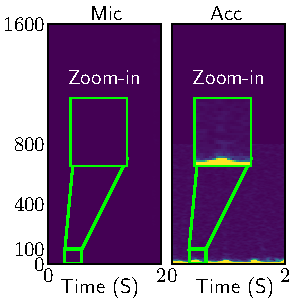
\includegraphics[width=1\textwidth]{chapters/vibvoice/figure/notalk.pdf}
        \caption{Spectrograms of microphone and acceleration when the user is walking.}
        \label{fig:vibvoice_walk}
\end{minipage}
\hfill
   \begin{minipage}[t]{0.48\columnwidth}
     \centering
       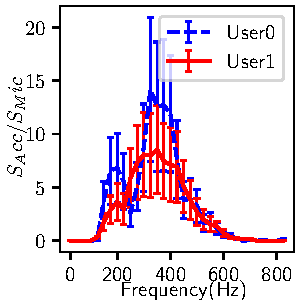
\includegraphics[width=1\textwidth]{chapters/vibvoice/figure/transfer_variance.pdf}
    \caption{Frequency responses of two users' bone-conducted vibrations.}
    %\vspace{-2em}
    \label{fig:vibvoice_bcf}
\end{minipage}
\end{figure}

\noindent\textbf{Frequency Response.}
We further explore the frequency response of bone-conducted vibrations among users. 
Specifically, we measure the frequency response as follows: first, we compute the spectra of audio and vibration data, denoted by $S_{\mathrm{Mic}}$ and $S_{\mathrm{Acc}}$, respectively. Then, we compute the Bone Conduction Function (BCF) as $S_{\mathrm{Acc}}/S_{\mathrm{Mic}}$ at every frequency band. Fig. \ref{fig:vibvoice_bcf} shows two volunteers' frequency responses, with error bars representing averages and variances.
Acceleration shows higher sensitivity than the microphone within $200$–$500\,\text{Hz}$, and lower sensitivity above $500\,\text{Hz}$ due to absorption by the skull. 
Additionally, the frequency response shows significant similarity among users, indicating generalization.
Hence, the BCF should consider inter-person diversity as well as inter-person similarity.

\begin{figure}
\begin{minipage}[t]{0.48\columnwidth}
     \centering
    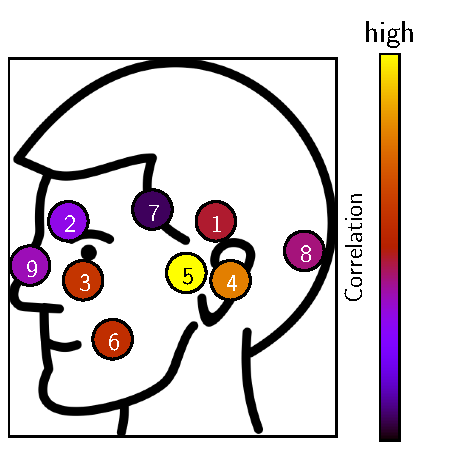
\includegraphics[width=\textwidth]{chapters/vibvoice/figure/correlation.pdf}
    \caption{Intensities of received bone-conducted vibrations on ten locations of the head.}
    \label{fig:vibvoice_head_positison}
\end{minipage}
\hfill
   \begin{minipage}[t]{0.48\columnwidth}
     \centering
    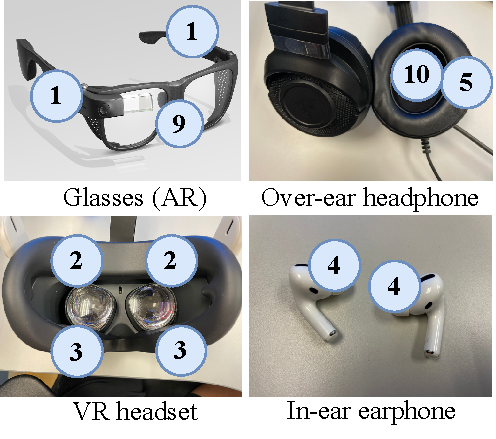
\includegraphics[width=\textwidth]{chapters/vibvoice/figure/devices.pdf}
    \caption{Potential placements on devices.}
    \label{fig:vibvoice_devices}
\end{minipage}
\end{figure}
\noindent\textbf{Locations on the head.}
Bone-conducted vibration exists at various locations on the head. 
As shown in Fig. \ref{fig:vibvoice_head_positison}, we select ten unique locations of interest on the head and measure the intensities of received bone-conducted vibrations. The nine facial/head locations are \#1 \emph{upper ear}, \#2 \emph{eyebrow}, \#3 \emph{cheekbones}, \#4 \emph{ear}, \#5 \emph{temporomandibular joint}, \#6 \emph{cheek}, \#7 \emph{temple}, \#8 \emph{back of the head}, and \#9 \emph{nose}. In addition, we tape EarSense on the interior of the pad of an over-ear headphone, denoted as \#10.
Among those positions, some are compatible with commercial HMWs like glasses, headphones, and VR headsets. Fig. \ref{fig:vibvoice_devices} illustrates the corresponding positions on HMWs. The numbers on the HMWs correspond to the locations in Fig. \ref{fig:vibvoice_head_positison}. 
We attach EarSense to the HMWs (when applicable) or on the face for all the following tests. 
We compute Pearson correlation coefficients between the audio and the acceleration on each location and mark the values using a color map in Fig. \ref{fig:vibvoice_head_positison}.
We observe that bone-conducted vibrations exist at most locations of the head. In particular, locations closer to the mouth show higher correlations, indicating a larger possibility of extracting clean speech. 

In summary, our measurements show that bone-conducted vibration has the following characteristics: a) it is robust to environmental voices and primarily captures the user's speech; b) user motion mainly generates vibrations lower than $85\,\text{Hz}$; c) it suppresses low- and high-frequency audio, with variations across and within users; and d) usable signals can be received from multiple locations on the head.

\subsection{Human Activity Recognition}
\label{sec:egolog_measurement}
As discussed in Sec. \ref{sec:egolog_intro}, multimodal HAR on mobile devices faces three main challenges: 1) lack of scenario awareness, 2) sensitivity to ambient noise, and 3) fusion collapse. To explore these challenges and assess potential solutions, we conduct a series of experiments.

\begin{figure}
    \centering
    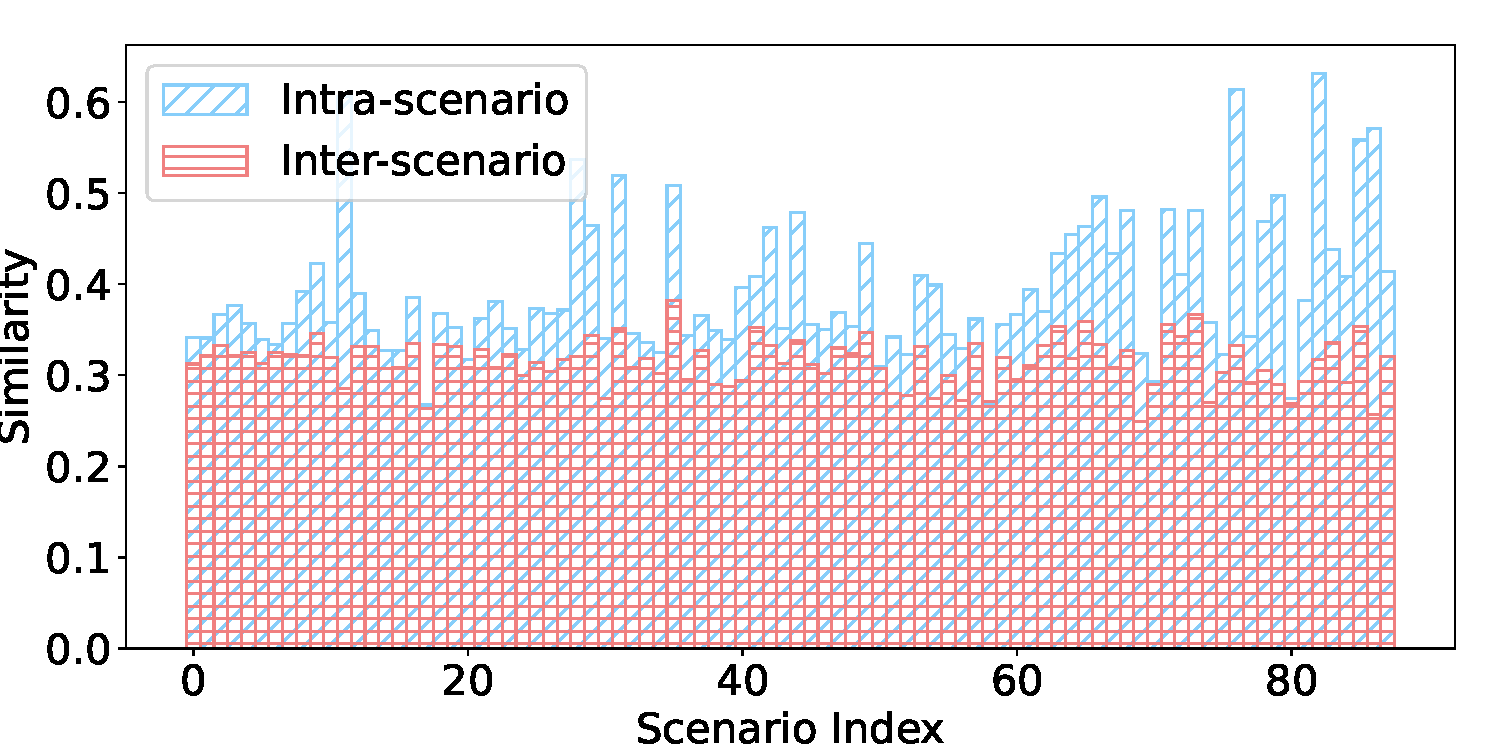
\includegraphics[width=0.8\linewidth]{chapters/egolog/figs/scenario_similarity.pdf}
    \vspace{-1em}
    \caption{Motivation for scenario understanding: 
    The similarity of embeddings for intra- and inter-scenario activities.}
    \label{fig:egolog_scenario_similarity}
    \vspace{-1em}
\end{figure}

\subsubsection{Scenario}
\label{subsec:scenario}
Scenario information refers to long-time activities (e.g., playing with a pet or working at home) that reflect the user's real-world behavior. Capturing such scenarios in datasets is challenging, as it requires volunteers to perform activities naturally, mimicking real-life conditions. Generally, scenario is the ensemble of multiple related and continuous activities with a realistic distribution, reflecting meaningful interactions with the environment.

To investigate the impact of scenario information on HAR, we utilize the Ego4D dataset \citep{grauman2022ego4d}, which captures real-world activities through smart glasses equipped with IMU and audio sensors. The dataset provides annotations at both the window level (every 10 seconds) and the video level, represented as plain text. We treat window-level annotations as activity labels and video-level annotations as scenario labels, reflecting prolonged activities. To examine scenario properties, we employ Sentence-BERT \citep{reimers2019sentence} to generate text embeddings for activities across 91 scenarios. We then compute activity similarity both within scenarios (intra-scenario) and between scenarios (inter-scenario). Intra-scenario similarity measures the similarity of activities within the same scenario, while inter-scenario similarity compares an activity from one scenario to a randomly selected activity from a different scenario.

The results in Fig.~\ref{fig:egolog_scenario_similarity} reveal that intra-scenario similarity is over 20\% higher than inter-scenario similarity. This suggests that each scenario has a distinct distribution of activities and effectively represents the user's daily log over a longer time frame.
Additionally, inter-scenario similarity is generally above 0.3, indicating that many basic activities (such as sitting and walking) are common across scenarios. Therefore, it is crucial to reduce the influence of these basic activities in scenario recognition.


In summary, the study on the in-the-wild dataset indicates unique activity distributions per scenario, which can be leveraged to recognize scenarios by identifying scenario-specific activities.

\subsubsection{Sound Location }
\label{subsec:embodied}
\begin{figure}
    \centering
    \begin{minipage}{0.48\linewidth}
        \centering
       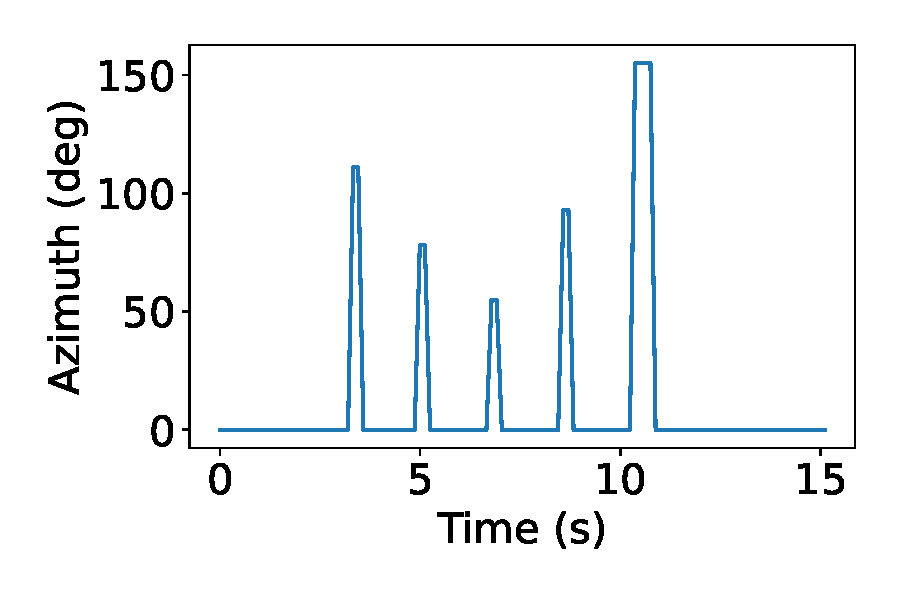
\includegraphics[width=\linewidth]{chapters/egolog/figs/baseline_result.pdf}
        \caption{Sound localization under motion \citep{schmidt1986multiple}}
        \label{fig:egolog_loc_move}
    \end{minipage}
    \hfill
    \begin{minipage}{0.48\linewidth}
        \centering
        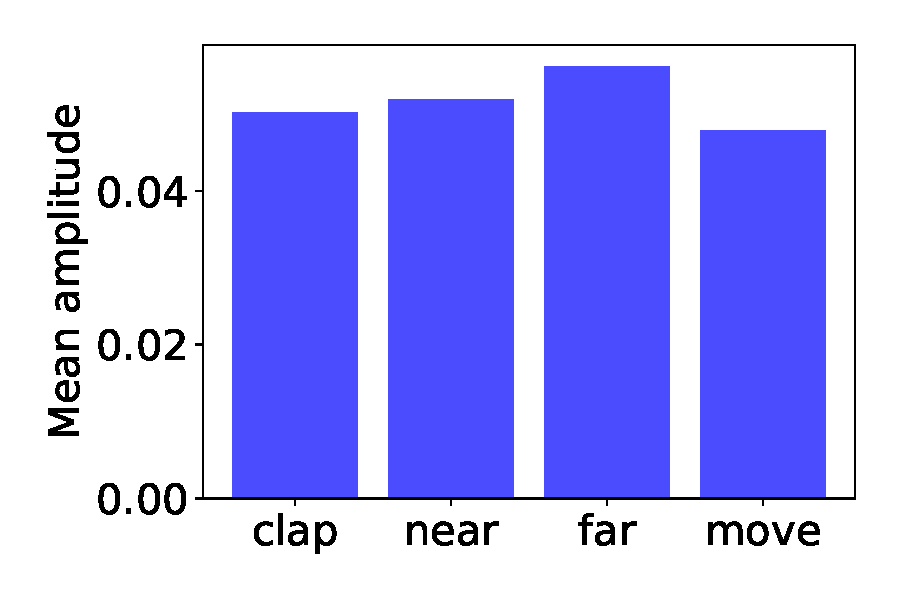
\includegraphics[width=\linewidth]{chapters/egolog/figs/amplitude.pdf}
        \caption{Sound volume may not relate to distance.}
        \label{fig:egolog_amplitude}
    \end{minipage}    
    \vspace{-1em}
\end{figure}

\begin{figure}
    \centering
    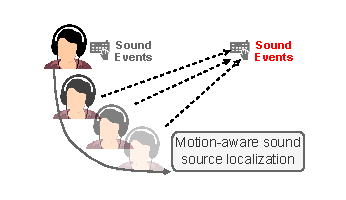
\includegraphics[width=0.75\linewidth]{chapters/egolog/figs/spatial_motivation.pdf}
    \vspace{-1em}
    \caption{Motivation for spatial understanding: estimate the distance of a sound event via motion.}
    \vspace{-1em}
    \label{fig:egolog_motivation_localization}
\end{figure}

In practice, recorded audio often includes far-field sound sources that are unrelated to the user’s activities, underscoring the importance of sound localization for effective HAR. Wearables that are consistently worn on the user’s head provide a stable and reliable position for capturing detailed ambient sound information. Additionally, modern wearables feature multi-channel recording capabilities, enhancing their spatial sensing potential.
In the following, we divide sound localization into direction and distance estimation, which we discuss as follows.

Estimating sound direction is mature but remains challenging. Accuracy depends heavily on the number of microphones, which is limited in most commercial devices. In common stereo settings, two main problems arise: directional deviation (especially front–back confusion) and estimating sound distance, as illustrated in Fig. \ref{fig:egolog_motivation_localization}.
We envision addressing these challenges via motion compensation. Specifically, we can aggregate consecutive localization results along with user (microphone) movement to refine direction estimates and infer distance.

To illustrate, we positioned a sound source in front of the user and utilized a binaural microphone along with the algorithm from \citep{schmidt1986multiple} to estimate direction of arrival, as shown in Fig. \ref{fig:egolog_loc_move}. The user was instructed to move slightly and naturally. Estimates were not satisfactory, fluctuating around the true value of 90 degrees. To validate whether sound volume differentiates near vs. far, we conducted an experiment with varying source distances. As shown in Fig. \ref{fig:egolog_amplitude}, there was no notable volume difference between cases, indicating that volume alone is an unreliable indicator of distance. The final bar in Fig. \ref{fig:egolog_amplitude} reveals that user movement slightly affects amplitude. Multiple sound sources can further complicate volume patterns.

\subsubsection{Multi-modal Fusion }
\label{subsec:measure-fuse}

\begin{figure}
    \centering
     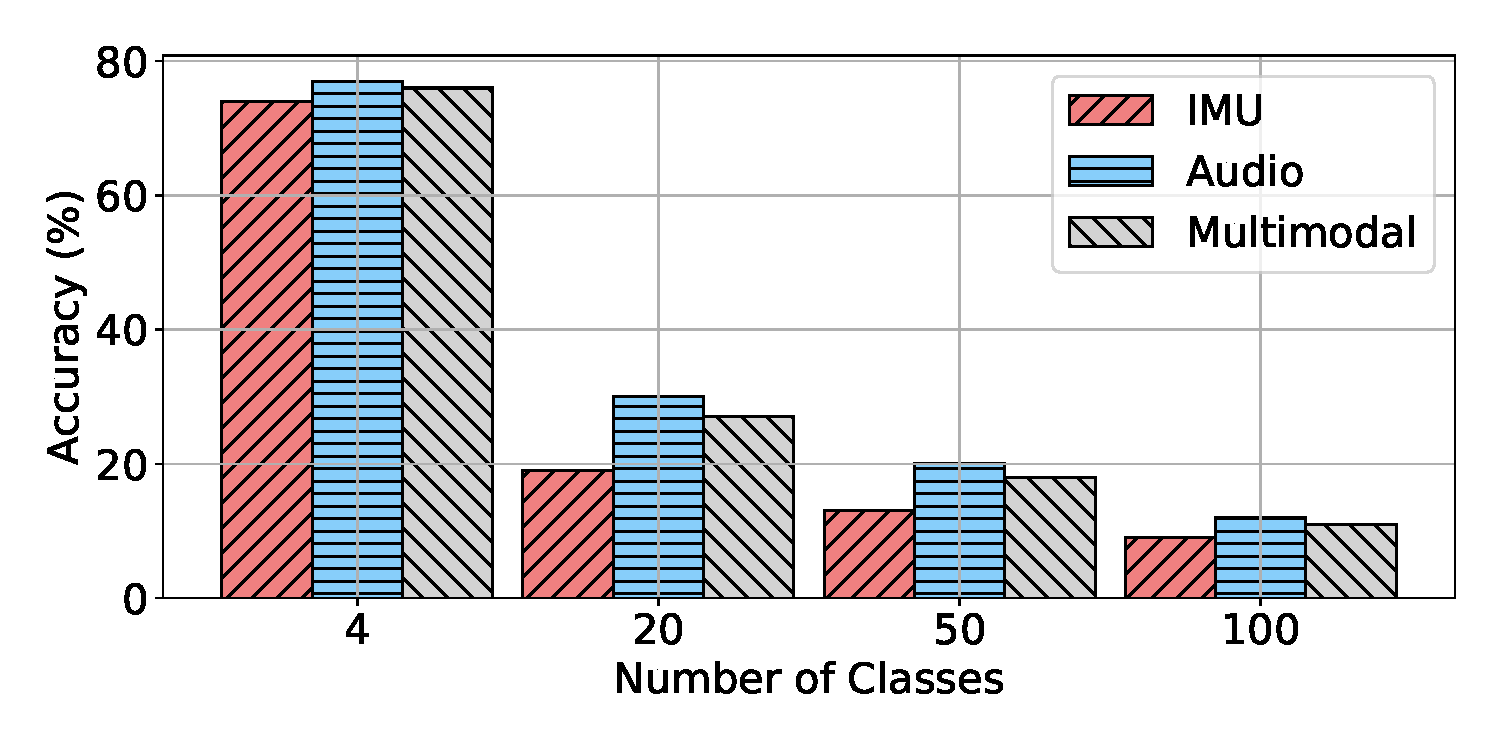
\includegraphics[width=.75\linewidth]{chapters/egolog/figs/num_class.pdf}
     \vspace{-1em}
      \caption{The performance of an existing activity recognition with different class numbers and modalities.}
    \label{fig:egolog_num_class}
    \vspace{-1em}
\end{figure}

To investigate scalability bottlenecks in activity recognition using wearables, we trained unimodal supervised models with audio and IMU data on the Ego4D episodic memory subset (200 activity classes). We used EfficientAT~\citep{schmid2023efficient} for audio and LIMU-BERT~\citep{xu2021limu} for IMU as feature extraction backbones, comparing them to a multi-modal model via late fusion. Activities were clustered into varying class numbers using Sentence-BERT~\citep{reimers2019sentence} embeddings and K-Means~\citep{macqueen1967some}, following MMG-Ego4D~\citep{gong2023mmg}. Results (Fig.~\ref{fig:egolog_num_class}) show a significant performance drop as class numbers increase, indicating challenges in recognizing diverse activities with audio or IMU alone. Multimodal fusion often underperforms unimodal models, suggesting ineffective extraction of complementary features at larger scales.

\begin{figure}
    \centering
    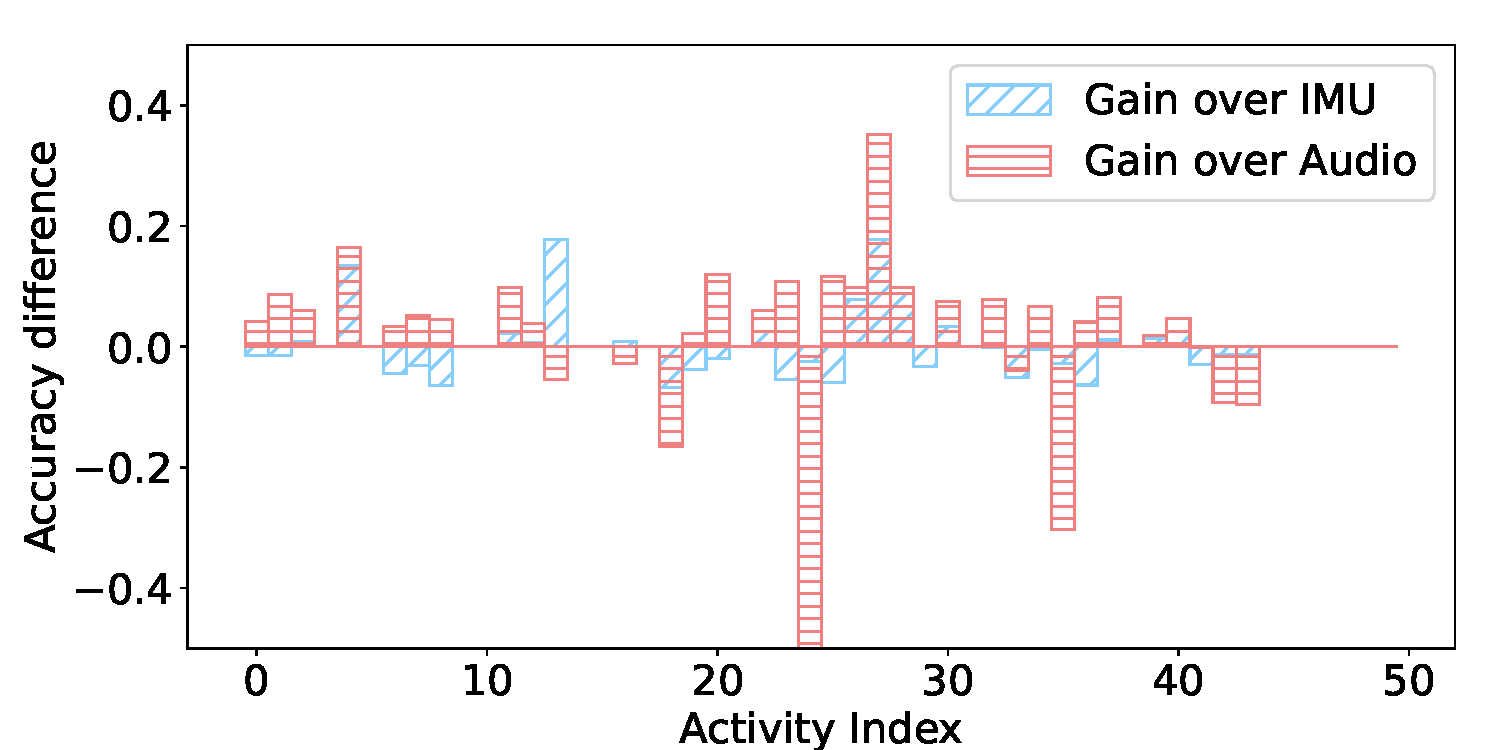
\includegraphics[width=.75\linewidth]{chapters/egolog/figs/activity_diff.pdf}
    \vspace{-1em}
    \caption{Performance gain from multi-modal fusion.}
    \label{fig:egolog_acc_gap}
    \vspace{-1em}
\end{figure}

Previous work~\citep{mollyn2022samosa} demonstrates that multimodal learning can outperform unimodal models due to complementary information.
However, this does not always apply: another study~\citep{gong2023mmg} finds multimodal audio+IMU learning on Ego4D can perform worse than single-modality solutions. To investigate, we compare the accuracy of multimodal and unimodal models for each class (Fig. \ref{fig:egolog_acc_gap}). We observe that the advantages of multimodal fusion fluctuate across classes and modalities, indicating that supervised multimodal learning does not automatically select the right modality and may fail to benefit from fusion.


To investigate the effectiveness of LLMs in alleviating the problem, we employ ImageBind-LLM \citep{han2023imagebind}, which converts both modalities into features and conditions them with text embeddings. We instruct the model with: "<sensor> According to the audio and IMU reading on the user's earphone, what is the user's activity?", where <sensor> refers to the placement of sensor features. Because LLM outputs can be random, we also add a prompt to force it to output one of the potential activities. To reduce complexity, we select the top 30 activities in the Ego4D episodic memory subset. The BERT scores of ImageBind-LLM are 0.04 (precision), 0.07 (recall), and 0.05 (F1), which are too low for practical use. Inspecting outputs suggests the LLM may not fully understand the fusion task.
Furthermore, we investigate whether fine-tuning can resolve the problem by training an adapter~\citep{zhang2023llamaadapter} for ImageBind-LLM. The adapted LLM achieves BERT scores of 0.47 (precision), 0.46 (recall), and 0.47 (F1). Although much improved, performance remains below usability and is far from practical.
